\chapter{Privacy-sensitive Acoustic Perception for Mobile Devices}
\label{chap:sound}

\section{Introduction}

Speech enabled technology is an increasingly popular element in consumer devices, as seen in Smartphones, Home Assistants etc.
 To provide speech enabled features, devices rely on listening to the ambient raw audio stream for keyword spotting.
 Applications listening to raw audio pose serious questions about conversational privacy and personal security for the end-user \cite{alwaysListening}.
 As an attempt to protect privacy, the speech enabled features have been restricted only to "native" applications written by the device manufacturer.


In this chapter, I present a solution to this problem in two phases.
 I discuss audio obfuscation techniques and examine the trade-off between privacy and keyword spotting performance.
 I also identify the best solution within our framework that maximizes both privacy and keyword spotting performance.
 I present performance results in the field from an Android application (\texttt{dBHound Keyphrase}).
 I also support my argument with human level cognition performance on obfuscated audio.
 Using this approach allows the entire suite of applications on a consumer device to provide keyword-enabled services while maintaining user privacy.
 This is achieved by openly broadcasting the obfuscated audio to the applications on the device.
 Since most user interaction with applications can be decomposed into keywords, I envision that this approach will lead to comprehensive speech-enabled services while maximizing end-user conversational privacy.



\section{Threat Model and Privacy Objectives}
\label{sec:threat_model}

I define the application context as interactions with mobile devices that involve directing speech toward the device.
 This agrees with typical usage patterns of mobile devices with regards to keyphrase recognition (Figure \ref{fig:keyphrase_application_context}).
 This definition for our application context allows us to leverage difference in the audio signal caused by the directionality of sound waves. 

\begin{figure}[!th]
\centering

\includegraphics[width=0.4\textwidth]{sound/talking-into-cell-phone.jpg}
\caption{Keyphrase Recognition Application Context}
\label{fig:keyphrase_application_context}
\end{figure}

\TODO{figure showing the difference in recorded audio when the phone is facing the user/away from the user or in the user's pocket or on the table etc.}

\TODO{figure showing the difference in recorded audio when the user is speaking into the mic in the headset as opposed to general speech.}


I choose a list of common keyphrases \ref{tab:common_keyphrases} for evaluating the "utility" (keyphrase spotting performance) of my solution.
 The ambient noise in the background while using the application can either be white noise or babble noise.
 I also analyze the effect the intensity of noise has on our keyword spotting performance.

I use the TED-LIUM speech corpus \cite{TEDLIUMCorpus} as a representatitve example of everday conversations in English.
 The corpus also has the advantage of providing English speech examples from speakers with varying accents.
 I also construct babble noise examples by randomly selecting and merging small audio segments from the TED-LIUM speech corpus, as well as borrowing audio snippets from other noise data sets.
 For keyphrase data, I have crowdsourced data acqusition through my Android app and have a rich set of examples for each keyword.
 \TODO{figure showing number of examples for each keyword and their distribution by male/female, native speaker/non-native speaker, quiet/noisy background}.
 More details on the data acquisition process is described in Section \ref{sec:system_design}.


\begin{table}
\centering
\begin{tabularx}{0.4\textwidth}{| l | l |}
okay google & call mom \\
hey siri & take a picture \\
hey cortana & play a song \\
nine one one & make a note \\
\end{tabularx}
\caption{Common keyphrases chosen for prototyping privacy-preserving algorithms}
\label{tab:common_keyphrases}
\end{table}


\subsection{Rogue Mobile Applications}

The user installs an application "A" on his mobile device to assist with a particular task.
 The application "A" provides a voice interface for everyday use and is granted access to the microphone.
 However, the application "A", however is malicious and records everyday conversations of the user and transmits the audio content to a remote database.
 An attacker uncovers sensitive information from the audio in the remote database using speech recognition.

This is a threat model when applications have access to raw audio data.

\subsection{Adversarial Database Queries}

The user installs an application "A" on his mobile device to assist with a particular task.
 The application "A" provides a voice interface for everyday use and is granted access to obfuscating audio that is sufficient for its voice interface.
 The obfuscated audio data is stored in a database to improve the voice interface of the application.
 An attacker has prior knowledge of a keyword whose presence/absence (binary query) would indicate sensitive information of value.
 The attacker uncovers some sensitive information with a sequence of binary queries using keyword spotting.


This is a threat model when applications have access to obfuscated audio data.





\section{dbHound: System Design}
\label{sec:system_design}

The dBHound app is designed to simulate a layer between the raw audio stream and voice-enabled mobile applications.
 The applications only receive the obfuscated audio stream for providing their voice-enabled features.
 Any application that requires access to raw audio needs to request for permission from the user every time (Figure \ref{fig:proposed_voice_command_arch}).


The dbHound system is composed of an Android application to interface with the user and collect audio data, and a backend server that obfuscates the audio based on the settings and returns the classification result.
 The app communicates with the backend server using a REST API.
 The app does not access any personal information and all the REST API calls are completely anonymous.
 The only personal information collected is what the user provides when volunteering training data for the dbHound classification system.


Figure \ref{fig:dbhound_submit} shows the screenshot of the \texttt{dbHound Keyphrase} \footnote{The app can be found on the Google Play Store at \url{https://play.google.com/store/apps/details?id=edu.wisc.cs.dbhound}} Android application for users to volunteer training data.
 Figure \ref{fig:dbhound_test} shows the screenshots of the db \texttt{dbHound Keyphrase} application for users to test the keyphrase recognition.
 If the "Classify and Incrementally Train" option is enabled, the trained models are "fine-tuned" based on the user audio and label specified.

\begin{figure}[!th]
\centering
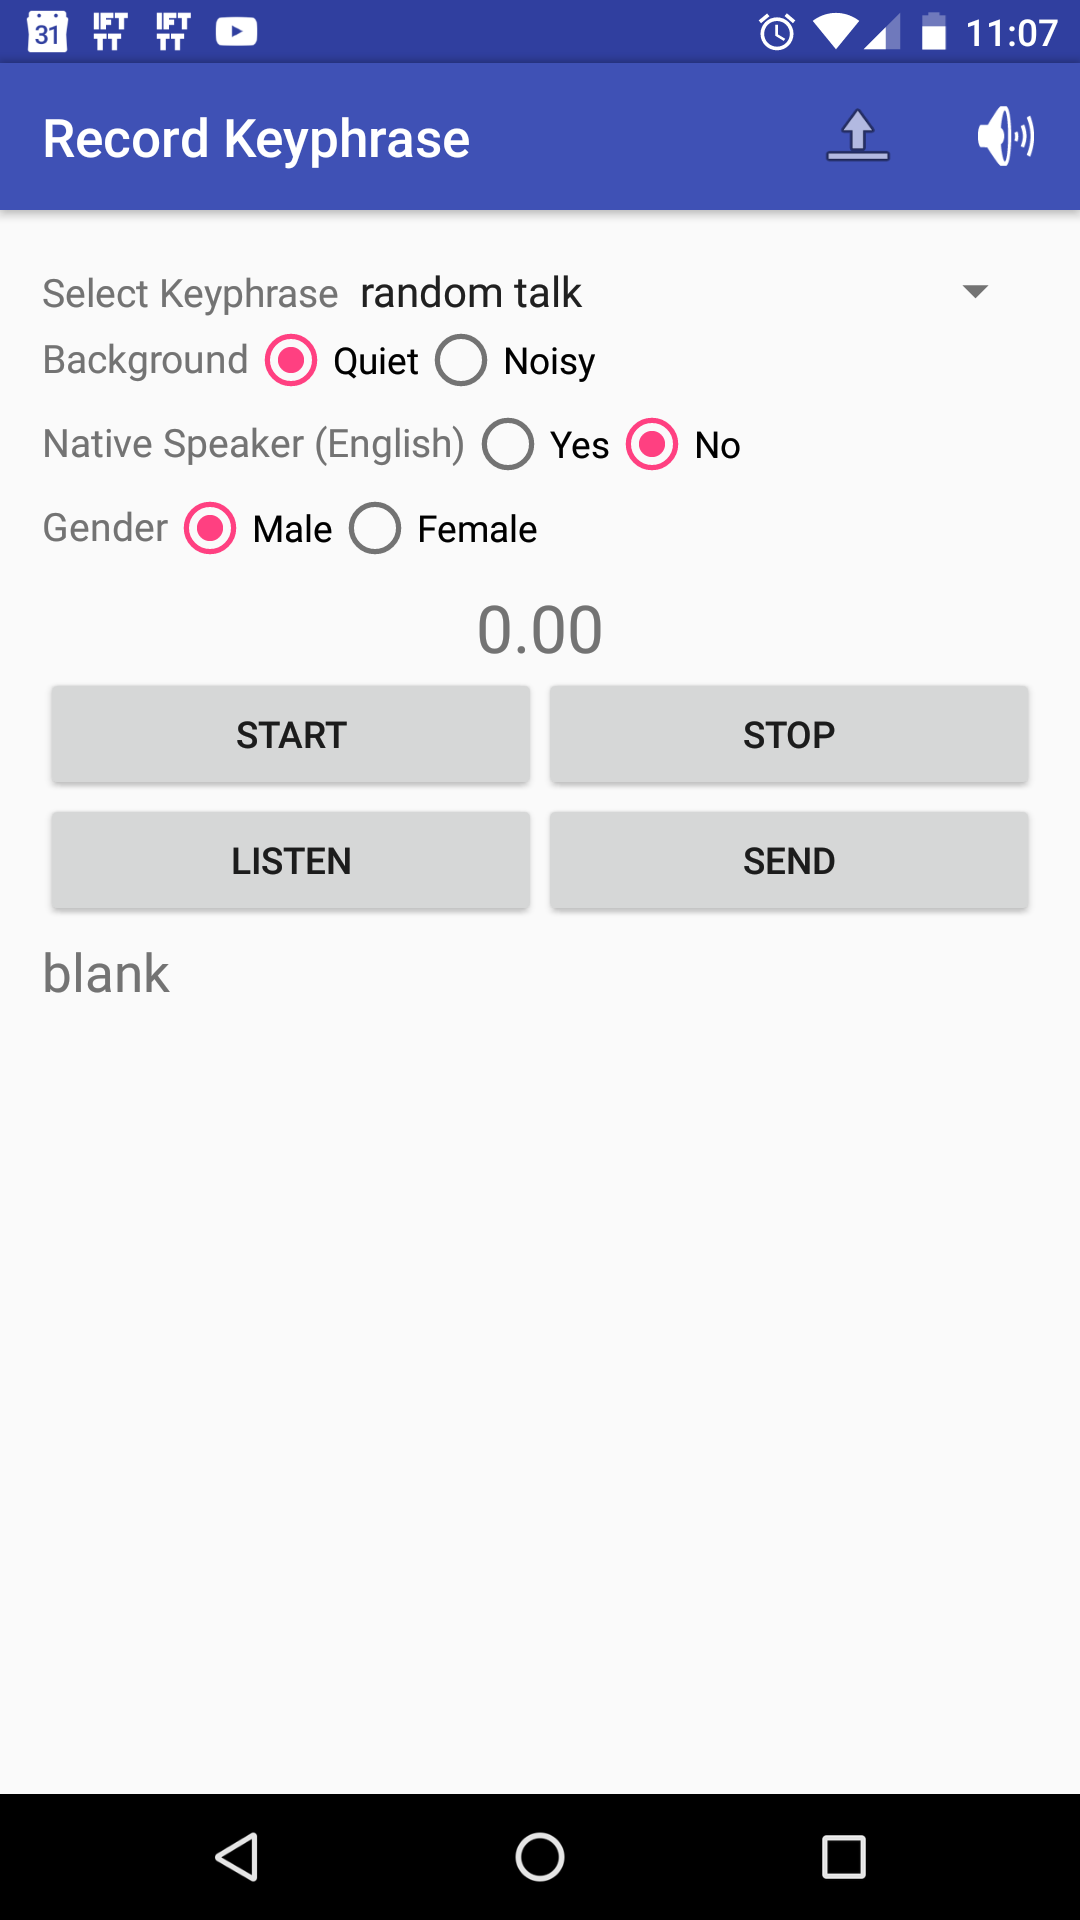
\includegraphics[width=0.25\textwidth]{sound/app_submit.png}
\caption{\texttt{dbHound Keyphrase} Android app screenshot for submitting training data}
\label{fig:dbhound_submit}
\end{figure}

\begin{figure}[!th]
\centering
\begin{subfigure}{0.5\textwidth}
\centering
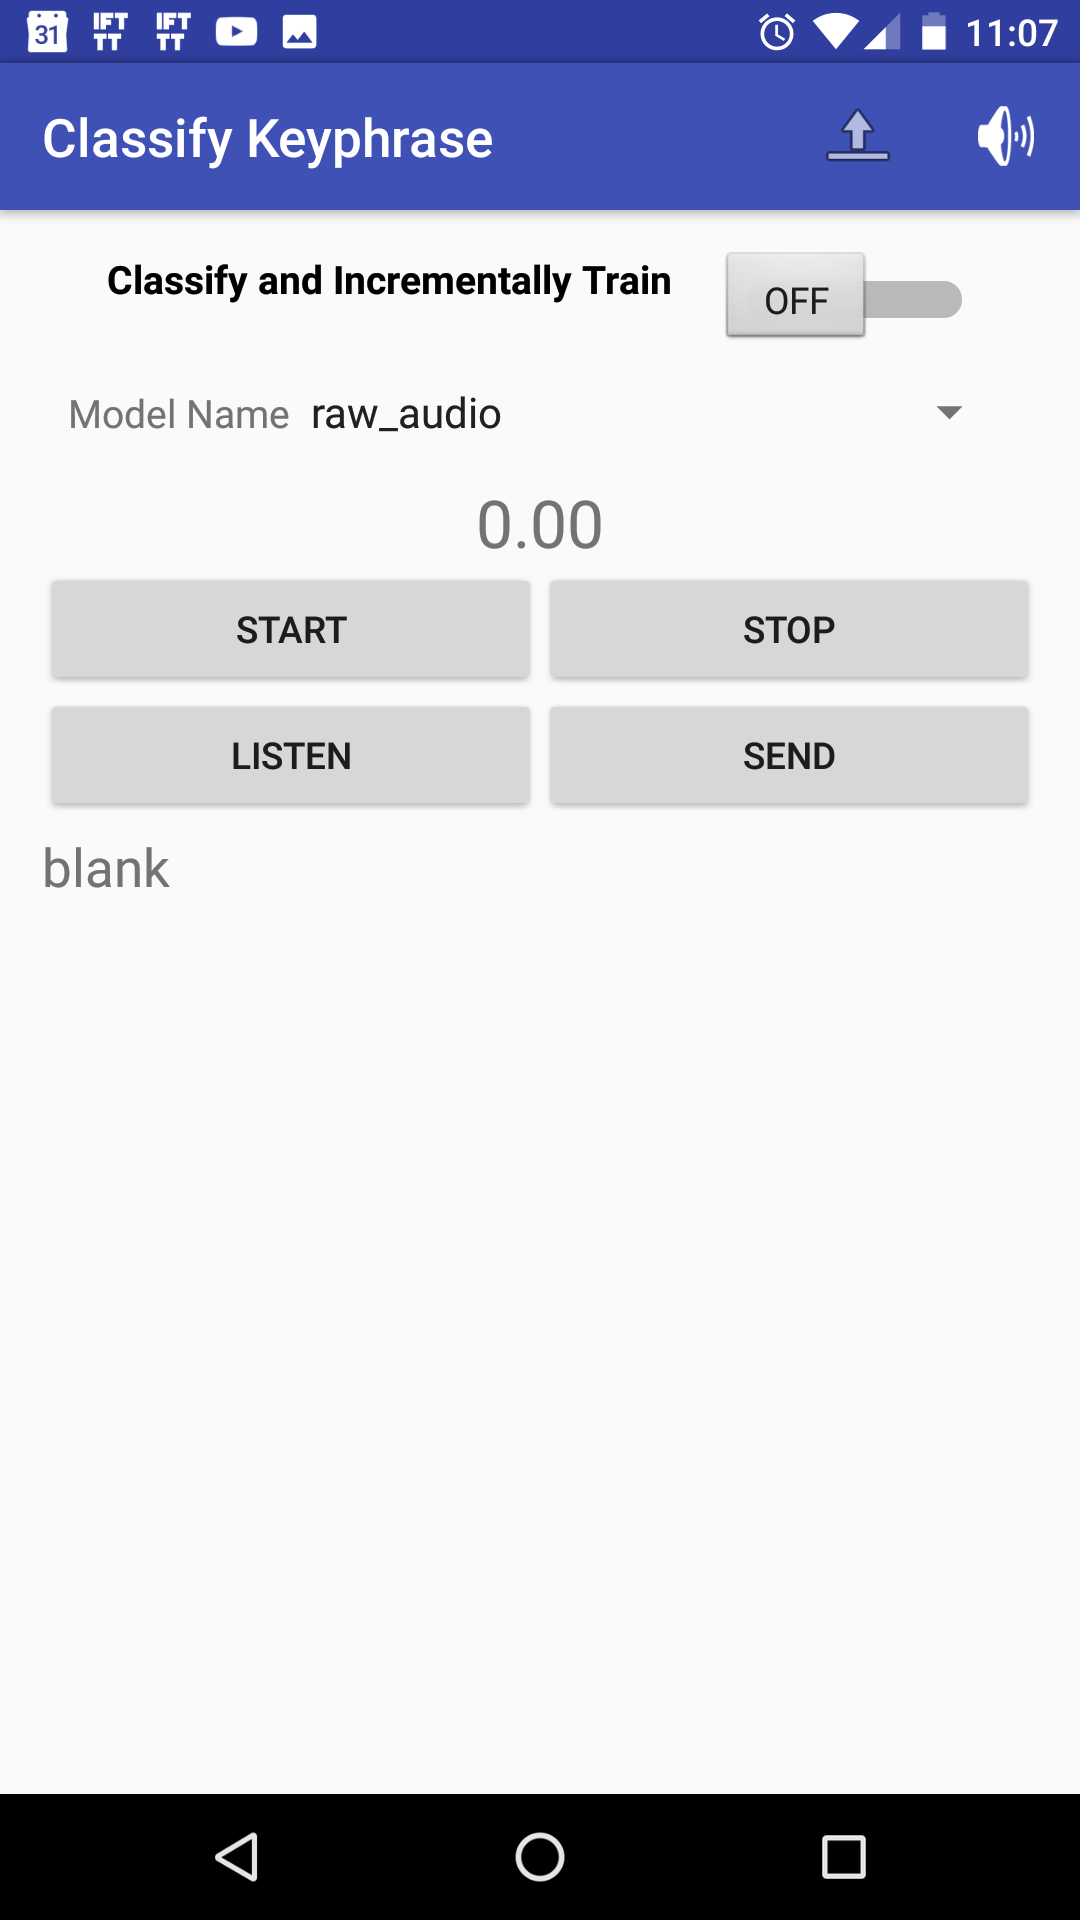
\includegraphics[width=0.5\textwidth]{sound/app_classify.png}
\caption{Only Classify}
\end{subfigure}%
\begin{subfigure}{0.5\textwidth}
\centering
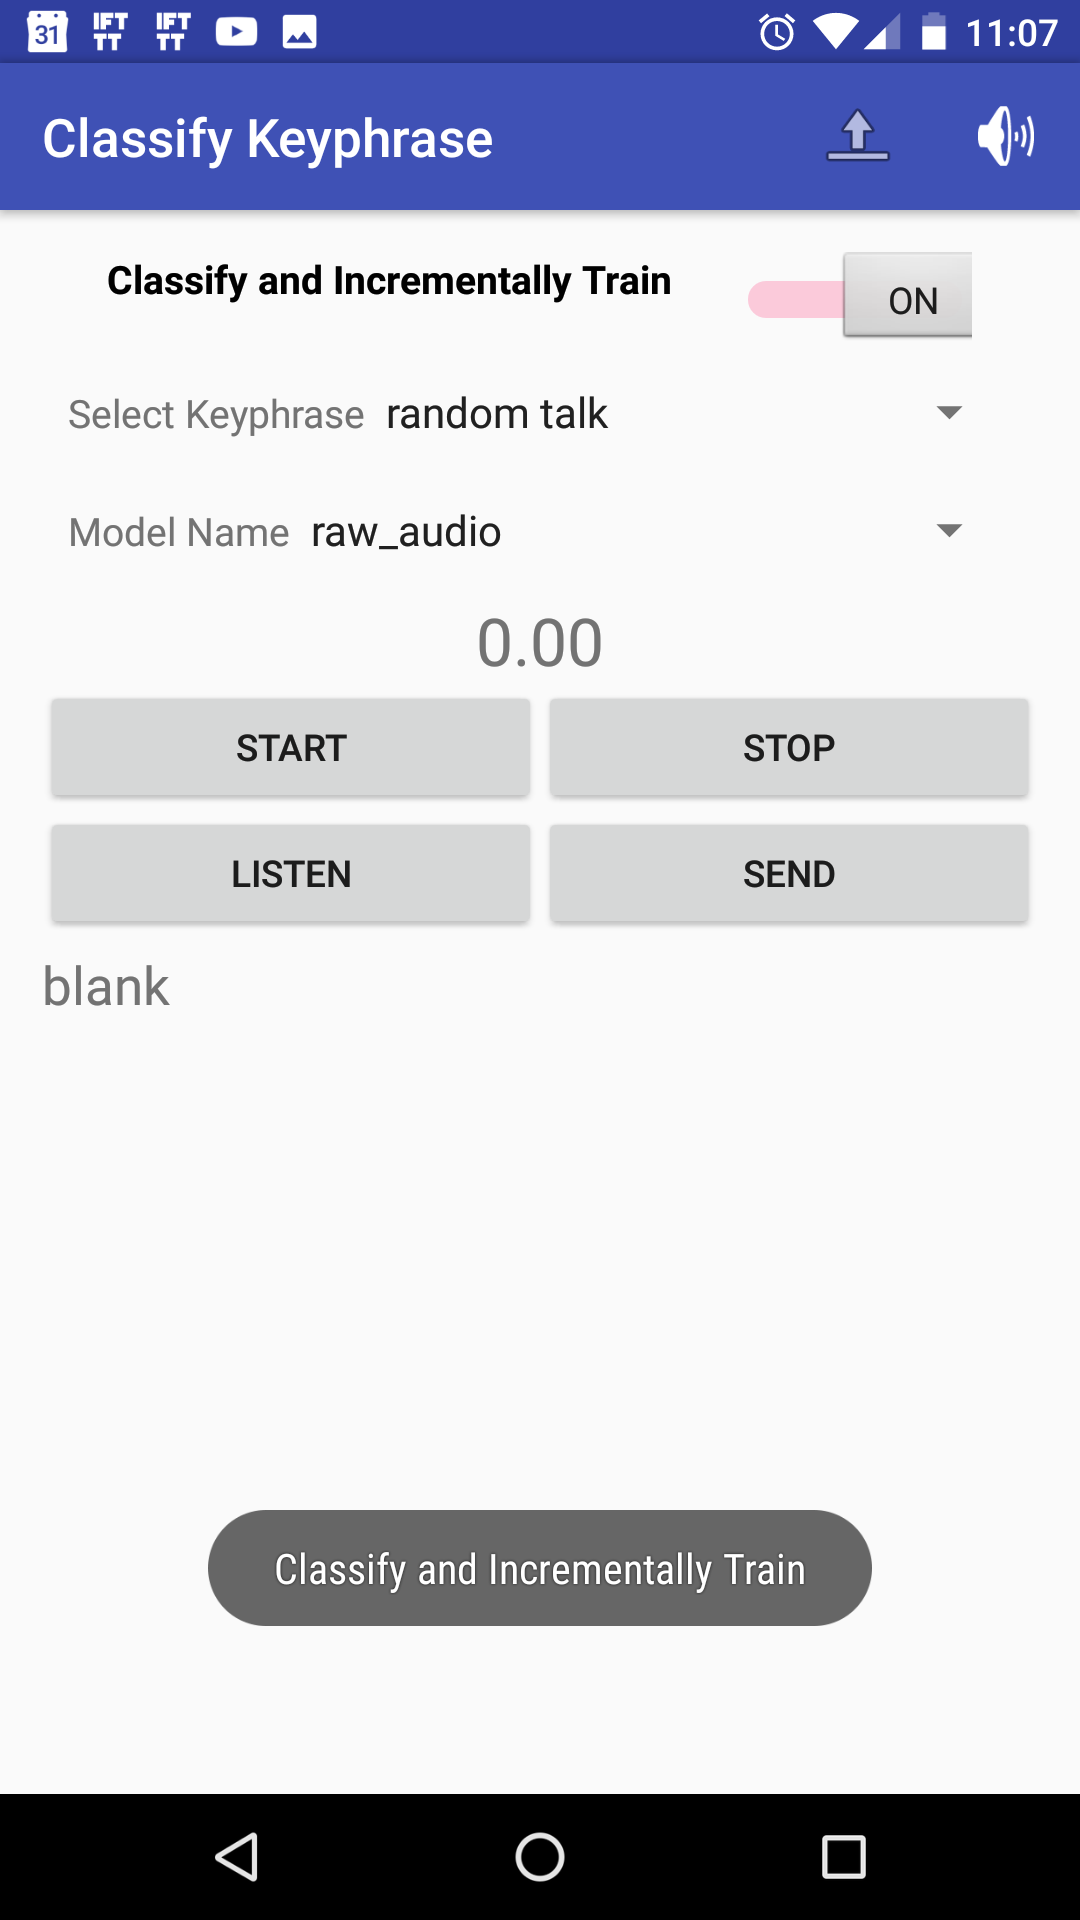
\includegraphics[width=0.5\textwidth]{sound/app_classify_and_train.png}
\caption{Classify and "Fine-Tune" Model}
\end{subfigure}%
\caption{\texttt{dbHound Keyphrase} Android app screenshot for testing the classification models}
\label{fig:dbhound_test}
\end{figure}

For preserving privacy, I propose a two-part solution:
\begin{itemize}
\item A computationally light transformation that removes conversational information from audio but preserves the ability to recognize a desired list of keywords.
\item A computationally light inference technique to spot the keywords from a stream of transformed audio data.
\end{itemize}





\section{Lightweight Audio Obfuscation}
\label{sec:obfuscation}

\TODO{small overview of both methods}

\TODO{describe data collected from mechanical turk in figure \ref{fig:mturk_survey}}. The first 4 bars correspond to decreasing decimated frequencies. \\ The last four bars correspond to decreasing bit depth of audio.

\afterpage{
    \begin{figure}[H]
    \centering
    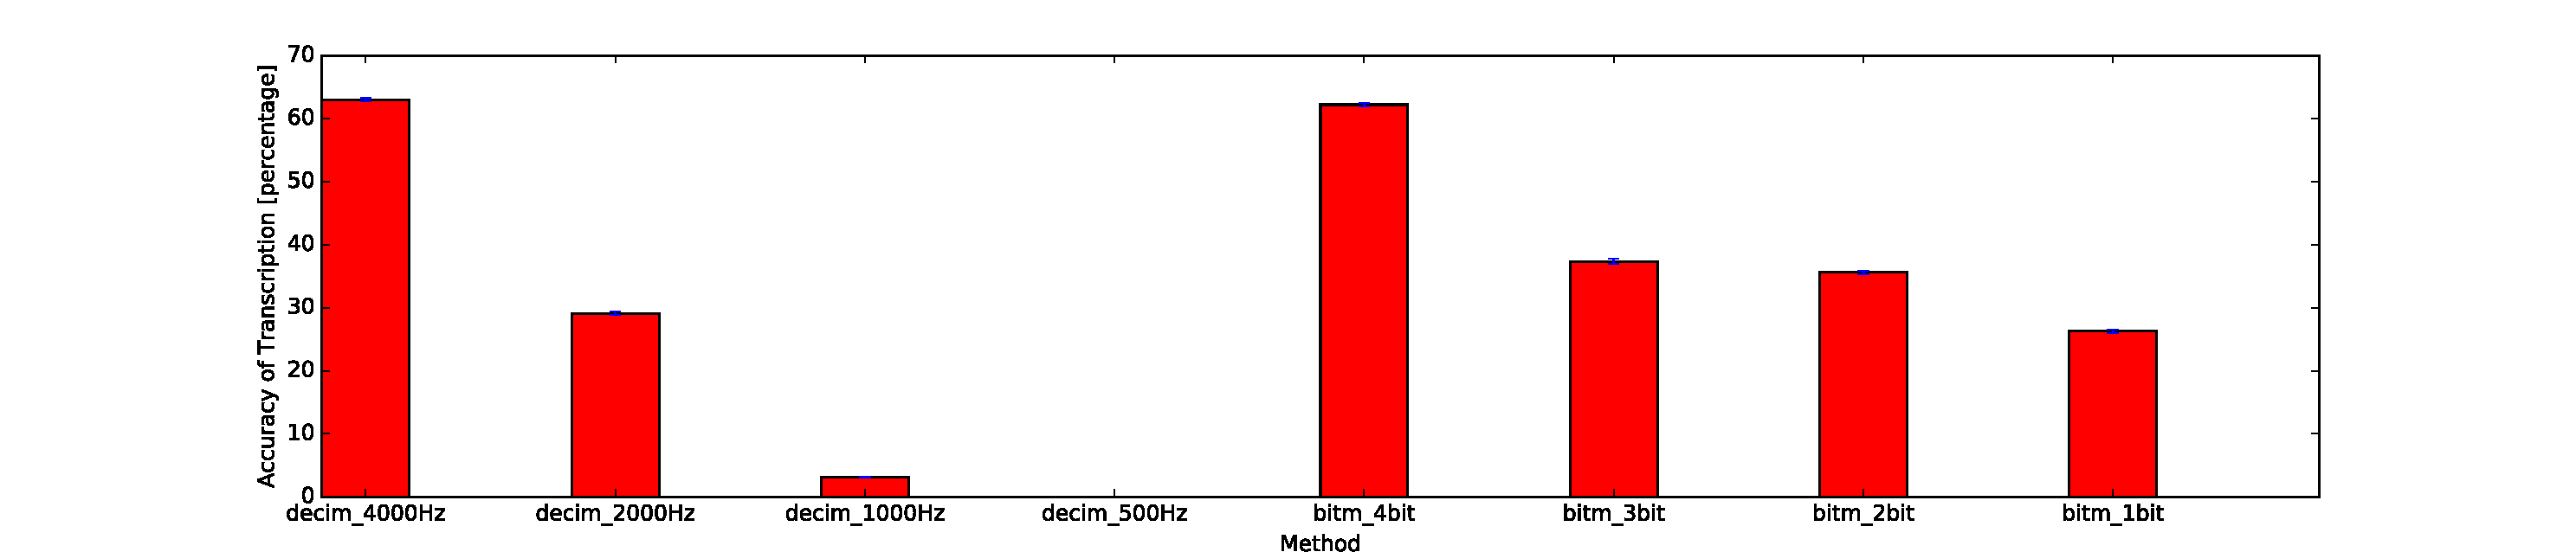
\includegraphics[width=\textwidth]{sound/mturk_survey.pdf}
    \caption{Accuracy of human transcription for different levels of decimation and quantization.}
    \label{fig:mturk_survey}
    \end{figure}
    \begin{table}[H]
    \begin{tabularx}{\textwidth}{l | l | l | l}
    \textbf{Key} & \textbf{Description} & \textbf{Key} & \textbf{Description} \\
    \hline
    decim\_4000 & Decimated to 4 kHZ & bitm\_4bit & 4-bit precision audio \\
    decim\_2000 & Decimated to 2 kHZ & bitm\_3bit & 3-bit precision audio \\
    decim\_1000 & Decimated to 1 kHZ & bitm\_2bit & 2-bit precision audio \\
    decim\_500 & Decimated to 500 HZ & bitm\_1bit & 1-bit precision audio \\
    \end{tabularx}
    \caption{Key for X-axis in Figure \ref{fig:mturk_survey}: \nameref{fig:mturk_survey}}
    \label{tab:key_mturk_survey}
    \end{table}
}

\subsection{Decimation: Removing time fidelity}

If the audio stream is recorded at 16kHz, we decimate the audio stream to a much lower sampling frequency.
 With this operation, the intelligibility of speech rapidly decreases with the amount of decimation.
 However, this also significantly decreases keyword spotting performance.

\TODO{ some raw data vs subsampled data? and the FFT for both to visualize information loss?}

\TODO{figure showing the performance decline of CMUSphinx, Google Speech Recog. with subsampled audio data}

\TODO{discuss the entropy and information content after this operation with respect to the raw audio}

\TODO{use differential privacy to discuss how adding controlled noise to this can prevent an attacker from understanding sensitive information.}


\subsection{Bit Depth: Removing amplitude fidelity}

If the audio stream is recorded at a 16-bit depth, we quantize the audio stream to a much lower bit depth to reduce the information content.
 Surprisingly, we find that, even at the lowest possible 1-bit depth, the speech content can be easily understood by humans (Figure \ref{fig:mturk_survey}).

\TODO{discuss: the loss of information with quantization? not so much}

\TODO{discuss the entropy and information content after this operation with respect to the raw audio}

\TODO{use differential privacy to discuss how adding controlled noise to this can prevent an attacker from understanding sensitive information.}

\subsection{Obfuscating audio using hamming weights}

If we consider each audio sample as one "sample bit", then we can compute the hamming weight of $n$ sample bits.
 This is done by concatenating the sample bit strings and counting the total number of "1"s in the $n$-sample bit string.

\TODO{discuss the entropy and information content after this operation with respect to the raw audio}

\TODO{use differential privacy to discuss how adding controlled noise to this can prevent an attacker from understanding sensitive information.}

\TODO{repeat the two analyses above applying the same hamming weight technique to both decimated audio and low bit-depth audio}

\subsection{Adding keywords to the dictionary}

\TODO{how would adding more keywords affect the privacy vs utility?}

\TODO{can we say if we add keywords with certain characteristics the algorithm will still be fine?}



\section{Keyphrase Recognition from Obfuscated Audio}
\label{sec:recognition_models}

I propose a deep neural network architecture (Figure \ref{fig:convnet_architecture}) to achieve this keyphrase recognition task in real time.
 Research work from Google in the past \cite{smallfootprintkeywordspotting} \cite{cnnkeywordspotting} \cite{chen2015locallyconnected} \cite{chen2014low} have shown that deep convolutional neural networks are suitable for online keyphrase recognition in mobile devices.
 The focus of my work is to survey the trade-off between privacy and keyphrase recognition performance for different audio obfuscation techniques.
 Based on the work from Google, I add the remark that efficient implementations of such architectures have been realized for mobile devices and it will be possible to translate the architecture I propose in a similar fashion, to mobile devices to realize the recommendations in Section \ref{sec:proposed_changes_to_mobile}.

The different layers of the deep convolutional neural network are described in detail below.

\subsection{Input Layer}

This contains all the samples from the obfuscated audio for a 2.048 second interval, with the audio being sampled at 16 kHz with 16-bit resolution.
 The interval of 2.048 seconds was chosen so that the corresponding number of raw audio samples is a power of 2 (32768 raw audio samples).
 This choice is purely one of convenience for signal processing.


Based on the obfuscation technique applied, the total number of samples provided in the input layer may be different.
 Some examples for this are shown in Table \ref{tab:input_layer_samples}.
 However, all of these variants still correspond to a time interval of 2.048 seconds, assisting in the consistency of the deep convolutional neural network across different obfuscation techniques.


For the sake of clarity when working with convolutional layers, the shape of the input layer can be re-written in the following manner.

\begin{gather}
\text{Shape Template} = (\text{height} \times \text{width} \times \text{channels}) \\
\text{Shape of Input Layer} = (N \times 1 \times 1)
\end{gather}

\begin{table}[!th]
\centering
\begin{tabularx}{\textwidth}{l | l}
\textbf{Obfuscation Technique} & \textbf{Input Layer Size} \\
\hline
No Obfuscation (Raw Audio) & 32768 \\
Decimation to 4 kHz & 8192 \\
Decimation to 1 kHz with 8-Hamming Reduction & 1024 \\
Decimation to 1 kHz & 2048 \\
Decimation to 1 kHz with 2-Hamming Reduction & 1024 \\
Bit Depth to 1 bit & 32768 \\
Bit Depth to 1 bit with 8-Hamming Reduction & 4096 \\
\end{tabularx}
\caption{Example list of size of input layer in the Deep Convolutional Neural Network for various obfuscation techniques}
\label{tab:input_layer_samples}
\end{table}

\subsection{Convolutional Layers}

In this case, I propose using 3 cascaded convolutional layers (interspersed with 3 max-pooling layers) to learn audio features for the classification task.
 Since the "width" (from the shape template above) is always 1, these layers can also be likened to a 1-D convolutional operation.
 Each convolutional layer is completely defined by the parameters described below. \footnote{Chris Olah's explanation in \cite{cnn_modular} is a great resource to understand the structure of ConvNets.}

\begin{itemize}
\item \textbf{Filter Size $(S)$:} The size of the convolutional filter defines the number of samples to work with to generate a feature.
 This also decides the size of the weight matrix for a single convolutional filter.
 For example, if only one filter of size $(20 \times 1 \times 1)$ is present, the filter works with 20 audio samples and 1 channel
 In other words, 20 weight variables are learnt per filter.
 The filter width is always 1, since this is a 1-D signal, and typically the filter works with all the channels of the input.
 Consequently, the filter size $S$ can be defined by a single number, 20, in this case.

\item \textbf{Filter Strides $(P)$:} The term "convolution" applies here because of the striding operation.
 Once the size of the convolutional filter is decided, the filter walks over sub-sections of the input space to compute a feature for different parts of the input.
 This can be likened to computing the Fourier Transform of different portions of a signal to understand localized frequency distributions --- the convolutional filter learns to find the best localized features.
 Clearly, given the high sample frequency of audio signals, striding the filter sample by sample would result in excessive computational time.
 Moreover, striding sample by sample is not likely to provide accuracy benefits either --- owing to the high sample frequency, the information (or phoneme) content is dispersed.
 The Filter Strides $P$ is the number of samples the filter "walks" over before computing the next feature.


Decreasing this parameter results in the filter striding in shorter steps (more instances of the same filter), increasing computation time while learning and evaluating.
 The size of the model (in terms of memory), however, remains unchanged.

\item \textbf{Number of Filters $(K)$:} This is used to set the number of filters (different features) to learn from the input.
 This can be likened to computing different types of transforms (e.g. fourier, haar, daubechies, cepstral etc.) over the same sub-sections of the input data.
 The intuition behind this is that different filters are likely to capture the essential features of the signal when used together.

\item \textbf{Activation Function:} This is the activation function used to generate the output at each node.
 Typical choices are ReLU, Sigmoid, tanh etc.

\end{itemize}

The size of the output of the 1-D convolutional filter is described below.
 The structure of my proposed deep convolutional neural network is described in \ref{tab:conv_layer_list}.

\begin{gather}
\text{Shape Template} = (\text{height} \times \text{width} \times \text{channels}) \\
\text{Shape of Input Layer} = (N \times 1 \times C) \\
\text{Shape of Output Layer} = \left(\frac{N-S+1}{P}, 1, K \right)
\end{gather}

The max-pooling layers are equivalent to a subsampling operation.
 They are introduced to maintain local translational invariance in the model.
 Consequently, a max-pooling operation of 4 decreases the number of input samples by a factor of $\left(\frac{1}{4}\right)$ in the output.
 The number 4 here is referred to as the "kernel size" of the max-pooling layer.
 It is standard practice for a max-pooling layer to follow a convolutional layer.
 \footnote{The Convolutional Layer together with its Max-Pooling Layer will be referred to as Conv-Max layer in the rest of this thesis.}
 All the max-pooling layers used in the architecture in Figure \ref{fig:convnet_architecture} have kernel size 2.

\begin{table}[!th]
\centering
\def\arraystretch{2}\tabcolsep=10pt

\begin{subtable}{\textwidth}
\centering
\begin{tabular}{l | l | l}
\textbf{Parameter} & \textbf{Convolutional Layer: 1} & \textbf{Convolutional Layer: 2} \\
\hline
Filter Size & $S = \frac{N}{128} \sim 16 ms$ & $S = 2 \sim 32 ms$ \\
Filter Strides & $P = \frac{S}{2} = \frac{N}{256}$ & $P = \frac{S}{2} = 1$ \\
Number of Filters & 1024 & 512 \\
Activation Function & ReLU & ReLU \\
Regularization & $L_2$ & $L_2$ \\
\end{tabular}
\end{subtable}

\vspace{3cm}

\begin{subtable}{\textwidth}
\centering
\begin{tabular}{l | l}
\textbf{Parameter} & \textbf{Convolutional Layer: 3} \\
\hline
Filter Size & $S = 8 \sim 256 ms$ \\
Filter Strides & $P = \frac{S}{2} = 4$ \\
Number of Filters & 128 \\
Activation Function & ReLU \\
Regularization & $L_2$ \\
\end{tabular}
\end{subtable}

\caption{Description of filter size for the Deep Convolutional Neural Network Architecture in Figure \ref{fig:convnet_architecture}. The input layer has $N$ samples.}
\label{tab:conv_layer_list}
\end{table}

\subsection{Densely Connected Layers}

The cascaded convolutional layers are used to learn the "best" features for the classification task at hand.
 The densely connected layers are intended to learn the actual classification task from the "best" features.
 If the output of the cascaded convolutional layers are considered as "features", then the rest of the network is a two-layer perceptron.
 In other words, the rest of the network can be treated as a neural network with one hidden layer and one output layer.

The hidden layer has ReLU activation with dropout regularization (the dropout probability is chosen as 0.8).
 The output layer has a softmax activation function to compute class probabilities.


When the neural network is fine-tuned online by the dbHound system, only the weights for the densely connected layers (two-layer perceptron) are updated.
 The reason only the two-layer perceptron is fine-tuned is to prevent overfitting on new data --- using this approach, the feature computation is "frozen" and the classification boundary is \textbf{slightly} nudged to accommodate new examples.
 This "incremental" learning is also done with a very small learning rate with the idea that the classifier is already well learnt and only needs to be slightly adapted to deal with new data.

\begin{figure}[!t]
\centering
\tikzset{%
    cascaded/.style={%
        general shadow={%
            shadow scale=1,
            shadow xshift=-1ex,
            shadow yshift=1ex,
            draw,
            thick,
            fill=white
        },
        general shadow={%
            shadow scale=1,
            shadow xshift=-.5ex,
            shadow yshift=.5ex,
            draw,
            thick,
            fill=white
        },
        fill=white,
        draw,
        thick,
        minimum width=1.5cm,
        minimum height=2cm
    }
}

\tikzstyle{vecArrowShort}=[thick,
                      shorten >= 5.5pt,
                      postaction={draw,line width=2pt, black, shorten >= 4.5pt}
]
\tikzstyle{vecArrow}=[thick,
                      postaction={draw,line width=2pt, black}
]

\tikzstyle{maxpool} = [rectangle, draw, fill=yellow!20, text centered, rounded corners]
\tikzstyle{conv} = [rectangle, draw, fill=blue!20, text centered, rounded corners, minimum height=4em, minimum width=20em]
\tikzstyle{shortline} = [draw, -latex', fill=black, vecArrowShort]
\tikzstyle{line} = [draw, -latex', fill=black, vecArrow]
\tikzstyle{dense} = [draw, ellipse,fill=red!20, minimum height=2em]
\tikzstyle{input} = [rectangle, draw, fill=green!20, text centered, sharp corners, minimum height=2em, minimum width=15em, align=center]
\tikzstyle{output} = [rectangle, draw, fill=green!20, text centered, sharp corners, minimum height=2em, minimum width=5em, align=center]

\begin{tikzpicture}[node distance = 2cm, auto]

% nodes
\node [input] (input) { $N \text{Audio Samples}$ };
\node [cascaded, conv, below of=input] (conv1) { $\text{1-D Convolutional Layer: 1}$ };
\node [maxpool, below of=conv1] (maxpool1) { Max-Pool Layer: 1 };
\node [cascaded, conv, below of=maxpool1] (conv2) { $\text{1-D Convolutional Layer: 2}$ };
\node [maxpool, below of=conv2] (maxpool2) { Max-Pool Layer: 2 };
\node [cascaded, conv, below of=maxpool2] (conv3) { $\text{1-D Convolutional Layer: 3}$ };
\node [maxpool, below of=conv3] (maxpool3) { Max-Pool Layer: 3 };
\node [dense, below of=maxpool3] (dense1) { $\text{Fully Connected Layer: 1}$ };
\node [dense, below of=dense1] (dense2) { $\text{Fully Connected Layer: 2}$ };
\node [output, below of=dense2] (output) { $(2 \times 1)$ softmax output };

%arrows
\path [shortline] (input) -- (conv1);
\path [line] (conv1) -- (maxpool1);
\path [shortline] (maxpool1) -- (conv2);
\path [line] (conv2) -- (maxpool2);
\path [shortline] (maxpool2) -- (conv3);
\path [line] (conv3) -- (maxpool3);
\path [line] (maxpool3) -- (dense1);
\path [line] (dense1) -- (dense2);
\path [line] (dense2) -- (output);

\end{tikzpicture}
\caption{Architecture of the Deep Convolutional Neural Network for Keyphrase Recognition}
\label{fig:convnet_architecture}
\end{figure}





\section{Evaluating Keyphrase Recognition Performance}
\label{sec:recognition_evaluation}

In this section, I present performance results for the ensemble of classification models learnt from keyphrase data.
 The model is organized as follows:

\begin{itemize}
\item An individiual classification model is learnt for every keyphrase apart from "random talk".
 The objective of the classification is to distinguish between the true keyphrase and "random talk".
\item For a test audio clip, all 8 classification models are used to get class probabilities for the associated keyphrase.
 The keyphrase with the maximum class probability is chosen and compared to a confidence threshold.
 If the class probability is greater or equal to than the confidence threshold, the classification output is the true keyphrase.
 If the class probability is lower than the confidence threshold, the classification output is "random talk".
\end{itemize}


Summarized in \cref{tab:probs_raw_audio,tab:probs_raw_audio_hamming_1,tab:probs_raw_audio_hamming_4,tab:probs_raw_audio_hamming_16,tab:probs_samplerate_2000,tab:probs_samplerate_1000,tab:probs_samplerate_2000_hamming_1,tab:probs_samplerate_1000_hamming_1,tab:probs_samplerate_2000_hamming_4,tab:probs_samplerate_1000_hamming_4,tab:probs_samplerate_2000_hamming_16,tab:probs_precision_1_hamming_1,tab:probs_precision_1_hamming_4,tab:probs_precision_1_hamming_16}
 are the mean class probabilities for different keyphrase audio examples using different keyphrase models.
 Each table corresponds to a different obfuscation technique, as noted in the caption.
 Each table corresponds to a different obfuscation technique.
 Each row corresponds to a classification model for a single keyphrase.
 Each column corresponds to audio examples for a single keyphrase, or audio examples for "random talk".
 The class probabilities in the table indicate the level to which the model has learnt the training set.


Examples for "random talk" are an assortment of choices from three sources:
\begin{itemize}
\item TED-LIUM Speech Corpus
\item Babble Noise Examples (Cafeteria noise, Public Transit Vehicle Noise)
\item "random talk" examples from the \texttt{dbHound Keyphrase}\footnote{The \texttt{dbHound Keyphrase} android application can be found on the Google Play Store at \url{https://play.google.com/store/apps/details?id=edu.wisc.cs.dbhound}.} android application
\end{itemize}

Figures \ref{fig:roc_raw_audio} \ref{fig:roc_samplerate} \ref{fig:roc_precision_bits} show the Receiver Operating Curves (ROC) for different obfuscation techniques.
 The Receiver Operating Curve shows the variation of the false positive ratio and true positive ratio when the confidence threshold for classification is varied.
 These curves help understand how well the model is likely to perform in real life.


\begin{table}[!th]
\begin{tabular}{cccccccccc}%
\hline%
None&\rotate{random talk}{70}&\rotate{okay google}{70}&\rotate{hey siri}{70}&\rotate{hey cortana}{70}&\rotate{nine one one}{70}&\rotate{call mom}{70}&\rotate{take a picture}{70}&\rotate{play a song}{70}&\rotate{make a note}{70}\\%
\hline%
okay google&0.01&\textbf{0.83}&0.01&0.01&0.0&0.0&0.01&0.0&0.01\\%
hey siri&0.01&0.05&\textbf{0.64}&0.01&0.0&0.0&0.09&0.03&0.02\\%
hey cortana&0.01&0.03&0.03&\textbf{0.66}&0.04&0.02&0.02&0.02&0.02\\%
nine one one&0.0&0.0&0.0&0.0&\textbf{0.83}&0.03&0.0&0.01&0.01\\%
call mom&0.01&0.0&0.01&0.06&0.03&\textbf{0.94}&0.0&0.05&0.0\\%
take a picture&0.01&0.02&0.03&0.01&0.0&0.0&\textbf{0.77}&0.0&0.01\\%
play a song&0.02&0.01&0.03&0.02&0.01&0.04&0.01&\textbf{0.71}&0.03\\%
make a note&0.02&0.03&0.02&0.02&0.01&0.03&0.03&0.01&\textbf{0.67}\\%
\hline%
\end{tabular}
\caption{Mean Class Probabilities from 350 audio examples. Each row corresponds to a different keyphrase classification model. Each column corresponds to a different keyphrase audio example. \emph{Obfuscation technique: no obfuscation}}
\label{tab:probs_raw_audio}
\end{table}



\begin{table}[!th]
\begin{tabular}{cccccccccc}%
\hline%
None&\rotate{random talk}{70}&\rotate{okay google}{70}&\rotate{hey siri}{70}&\rotate{hey cortana}{70}&\rotate{nine one one}{70}&\rotate{call mom}{70}&\rotate{take a picture}{70}&\rotate{play a song}{70}&\rotate{make a note}{70}\\%
\hline%
okay google&0.07&\textbf{0.52}&0.06&0.12&0.09&0.1&0.08&0.08&0.1\\%
hey siri&0.1&0.14&\textbf{0.53}&0.14&0.12&0.09&0.14&0.13&0.11\\%
hey cortana&0.06&0.09&0.08&\textbf{0.58}&0.07&0.08&0.11&0.08&0.11\\%
nine one one&0.02&0.04&0.04&0.03&\textbf{0.77}&0.12&0.02&0.08&0.05\\%
call mom&0.01&0.01&0.03&0.04&0.05&\textbf{0.83}&0.02&0.1&0.06\\%
take a picture&0.01&0.05&0.03&0.07&0.06&0.03&\textbf{0.38}&0.09&0.05\\%
play a song&0.0&0.01&0.01&0.03&0.03&0.05&0.01&\textbf{0.39}&0.02\\%
make a note&0.04&0.06&0.08&0.06&0.1&0.08&0.05&0.08&\textbf{0.44}\\%
\hline%
\end{tabular}
\caption{Mean Class Probabilities from 350 audio examples. Each row corresponds to a different keyphrase classification model. Each column corresponds to a different keyphrase audio example. \emph{Obfuscation technique: hamming reduction on every 1 sample}}
\label{tab:probs_raw_audio_hamming_1}
\end{table}





\begin{table}[!th]
\begin{tabular}{cccccccccc}%
\hline%
None&\rotate{random talk}{70}&\rotate{okay google}{70}&\rotate{hey siri}{70}&\rotate{hey cortana}{70}&\rotate{nine one one}{70}&\rotate{call mom}{70}&\rotate{take a picture}{70}&\rotate{play a song}{70}&\rotate{make a note}{70}\\%
\hline%
okay google&0.04&\textbf{0.79}&0.06&0.12&0.03&0.03&0.07&0.05&0.05\\%
hey siri&0.06&0.07&\textbf{0.45}&0.08&0.04&0.05&0.07&0.04&0.05\\%
hey cortana&0.01&0.07&0.04&\textbf{0.57}&0.01&0.02&0.08&0.03&0.05\\%
nine one one&0.02&0.03&0.04&0.03&\textbf{0.64}&0.15&0.02&0.07&0.03\\%
call mom&0.0&0.0&0.02&0.02&0.05&\textbf{0.71}&0.01&0.05&0.05\\%
take a picture&0.03&0.05&0.02&0.05&0.01&0.01&\textbf{0.63}&0.02&0.02\\%
play a song&0.04&0.05&0.07&0.06&0.13&0.1&0.06&\textbf{0.32}&0.09\\%
make a note&0.0&0.01&0.01&0.02&0.02&0.03&0.02&0.04&\textbf{0.52}\\%
\hline%
\end{tabular}
\caption{Mean Class Probabilities from 350 audio examples. Each row corresponds to a different keyphrase classification model. Each column corresponds to a different keyphrase audio example. \emph{Obfuscation technique: hamming reduction on every 4 samples}}
\label{tab:probs_raw_audio_hamming_4}
\end{table}





\begin{table}[!th]
\begin{tabular}{cccccccccc}%
\hline%
None&\rotate{random talk}{70}&\rotate{okay google}{70}&\rotate{hey siri}{70}&\rotate{hey cortana}{70}&\rotate{nine one one}{70}&\rotate{call mom}{70}&\rotate{take a picture}{70}&\rotate{play a song}{70}&\rotate{make a note}{70}\\%
\hline%
okay google&0.03&\textbf{0.85}&0.0&0.09&0.0&0.0&0.01&0.0&0.0\\%
hey siri&0.0&0.0&\textbf{0.99}&0.0&0.0&0.0&0.0&0.0&0.0\\%
hey cortana&0.01&0.02&0.02&\textbf{0.91}&0.01&0.01&0.0&0.02&0.03\\%
nine one one&0.01&0.0&0.0&0.01&\textbf{0.98}&0.0&0.0&0.01&0.0\\%
call mom&0.0&0.0&0.01&0.0&0.0&\textbf{0.81}&0.0&0.01&0.0\\%
take a picture&0.0&0.0&0.0&0.0&0.0&0.0&\textbf{0.7}&0.0&0.0\\%
play a song&0.0&0.0&0.0&0.01&0.01&0.01&0.0&\textbf{0.68}&0.0\\%
make a note&0.02&0.0&0.0&0.0&0.0&0.0&0.0&0.0&\textbf{0.87}\\%
\hline%
\end{tabular}
\caption{Mean Class Probabilities from 350 audio examples. Each row corresponds to a different keyphrase classification model. Each column corresponds to a different keyphrase audio example. \emph{Obfuscation technique: hamming reduction on every 16 samples}}
\label{tab:probs_raw_audio_hamming_16}
\end{table}



\clearpage


\begin{table}[!th]
\begin{tabular}{cccccccccc}%
\hline%
None&\rotate{random talk}{70}&\rotate{okay google}{70}&\rotate{hey siri}{70}&\rotate{hey cortana}{70}&\rotate{nine one one}{70}&\rotate{call mom}{70}&\rotate{take a picture}{70}&\rotate{play a song}{70}&\rotate{make a note}{70}\\%
\hline%
okay google&0.03&\textbf{0.73}&0.03&0.02&0.01&0.0&0.05&0.01&0.02\\%
hey siri&0.01&0.03&\textbf{0.51}&0.03&0.01&0.02&0.05&0.02&0.03\\%
hey cortana&0.02&0.05&0.03&\textbf{0.74}&0.02&0.02&0.05&0.03&0.01\\%
nine one one&0.04&0.03&0.02&0.07&\textbf{0.87}&0.04&0.03&0.03&0.02\\%
call mom&0.0&0.0&0.02&0.02&0.04&\textbf{0.92}&0.0&0.08&0.02\\%
take a picture&0.02&0.02&0.04&0.01&0.0&0.0&\textbf{0.49}&0.01&0.01\\%
play a song&0.01&0.01&0.1&0.04&0.03&0.13&0.01&\textbf{0.81}&0.04\\%
make a note&0.04&0.06&0.03&0.03&0.04&0.03&0.02&0.04&\textbf{0.58}\\%
\hline%
\end{tabular}
\caption{Mean Class Probabilities from 350 audio examples. Each row corresponds to a different keyphrase classification model. Each column corresponds to a different keyphrase audio example. \emph{Obfuscation technique: samplerate reduced to 2000 Hz}}
\label{tab:probs_samplerate_2000}
\end{table}







\begin{table}[!th]
\begin{tabular}{cccccccccc}%
\hline%
None&\rotate{random talk}{70}&\rotate{okay google}{70}&\rotate{hey siri}{70}&\rotate{hey cortana}{70}&\rotate{nine one one}{70}&\rotate{call mom}{70}&\rotate{take a picture}{70}&\rotate{play a song}{70}&\rotate{make a note}{70}\\%
\hline%
okay google&0.01&\textbf{0.34}&0.01&0.03&0.01&0.01&0.02&0.01&0.03\\%
hey siri&0.06&0.06&\textbf{0.06}&0.06&0.06&0.06&0.06&0.06&0.06\\%
hey cortana&0.01&0.04&0.07&\textbf{0.68}&0.03&0.01&0.03&0.08&0.04\\%
nine one one&0.01&0.01&0.02&0.01&\textbf{0.64}&0.02&0.02&0.02&0.01\\%
call mom&0.01&0.02&0.02&0.06&0.04&\textbf{0.62}&0.01&0.03&0.02\\%
take a picture&0.05&0.05&0.05&0.05&0.05&0.05&\textbf{0.05}&0.05&0.05\\%
play a song&0.04&0.05&0.11&0.03&0.09&0.11&0.03&\textbf{0.66}&0.06\\%
make a note&0.02&0.04&0.03&0.08&0.03&0.02&0.06&0.06&\textbf{0.26}\\%
\hline%
\end{tabular}
\caption{Mean Class Probabilities from 350 audio examples. Each row corresponds to a different keyphrase classification model. Each column corresponds to a different keyphrase audio example. \emph{Obfuscation technique: samplerate reduced to 1000 Hz}}
\label{tab:probs_samplerate_1000}
\end{table}





\begin{table}[!th]
\begin{tabular}{cccccccccc}%
\hline%
None&\rotate{random talk}{70}&\rotate{okay google}{70}&\rotate{hey siri}{70}&\rotate{hey cortana}{70}&\rotate{nine one one}{70}&\rotate{call mom}{70}&\rotate{take a picture}{70}&\rotate{play a song}{70}&\rotate{make a note}{70}\\%
\hline%
okay google&0.03&\textbf{0.49}&0.05&0.06&0.03&0.02&0.04&0.02&0.02\\%
hey siri&0.07&0.07&\textbf{0.43}&0.1&0.1&0.1&0.09&0.1&0.07\\%
hey cortana&0.02&0.06&0.04&\textbf{0.44}&0.01&0.01&0.06&0.01&0.02\\%
nine one one&0.03&0.04&0.05&0.04&\textbf{0.72}&0.16&0.02&0.09&0.04\\%
call mom&0.01&0.0&0.02&0.02&0.03&\textbf{0.55}&0.02&0.04&0.06\\%
take a picture&0.06&0.05&0.04&0.06&0.01&0.01&\textbf{0.63}&0.03&0.02\\%
play a song&0.01&0.0&0.01&0.01&0.05&0.07&0.01&\textbf{0.43}&0.05\\%
make a note&0.01&0.03&0.04&0.05&0.04&0.07&0.04&0.04&\textbf{0.42}\\%
\hline%
\end{tabular}
\caption{Mean Class Probabilities from 350 audio examples. Each row corresponds to a different keyphrase classification model. Each column corresponds to a different keyphrase audio example. \emph{Obfuscation technique: samplerate reduced to 2000 Hz followed by hamming reduction on every 1 sample}}
\label{tab:probs_samplerate_2000_hamming_1}
\end{table}








\begin{table}[!th]
\begin{tabular}{cccccccccc}%
\hline%
None&\rotate{random talk}{70}&\rotate{okay google}{70}&\rotate{hey siri}{70}&\rotate{hey cortana}{70}&\rotate{nine one one}{70}&\rotate{call mom}{70}&\rotate{take a picture}{70}&\rotate{play a song}{70}&\rotate{make a note}{70}\\%
\hline%
okay google&0.05&\textbf{0.86}&0.03&0.09&0.03&0.05&0.03&0.04&0.03\\%
hey siri&0.03&0.01&\textbf{0.96}&0.03&0.03&0.02&0.04&0.01&0.06\\%
hey cortana&0.01&0.01&0.01&\textbf{0.51}&0.01&0.01&0.01&0.01&0.01\\%
nine one one&0.0&0.0&0.0&0.0&\textbf{1.0}&0.0&0.0&0.0&0.0\\%
call mom&0.01&0.0&0.01&0.0&0.0&\textbf{0.99}&0.0&0.01&0.0\\%
take a picture&0.01&0.05&0.01&0.03&0.01&0.02&\textbf{0.87}&0.01&0.03\\%
play a song&0.02&0.0&0.0&0.0&0.03&0.0&0.01&\textbf{0.9}&0.0\\%
make a note&0.0&0.0&0.0&0.0&0.0&0.0&0.0&0.0&\textbf{1.0}\\%
\hline%
\end{tabular}
\caption{Mean Class Probabilities from 350 audio examples. Each row corresponds to a different keyphrase classification model. Each column corresponds to a different keyphrase audio example. \emph{Obfuscation technique: samplerate reduced to 1000 Hz followed by hamming reduction on every 1 sample}}
\label{tab:probs_samplerate_1000_hamming_1}
\end{table}









\begin{table}[!th]
\begin{tabular}{cccccccccc}%
\hline%
None&\rotate{random talk}{70}&\rotate{okay google}{70}&\rotate{hey siri}{70}&\rotate{hey cortana}{70}&\rotate{nine one one}{70}&\rotate{call mom}{70}&\rotate{take a picture}{70}&\rotate{play a song}{70}&\rotate{make a note}{70}\\%
\hline%
okay google&0.01&\textbf{0.84}&0.01&0.01&0.02&0.01&0.01&0.02&0.01\\%
hey siri&0.0&0.0&\textbf{0.99}&0.0&0.0&0.0&0.0&0.0&0.0\\%
hey cortana&0.04&0.04&0.06&\textbf{0.78}&0.01&0.0&0.04&0.02&0.03\\%
nine one one&0.01&0.0&0.0&0.04&\textbf{0.91}&0.0&0.01&0.02&0.01\\%
call mom&0.0&0.0&0.0&0.0&0.0&\textbf{0.28}&0.0&0.0&0.0\\%
take a picture&0.0&0.0&0.0&0.0&0.0&0.0&\textbf{1.0}&0.0&0.0\\%
play a song&0.01&0.0&0.0&0.0&0.0&0.0&0.0&\textbf{0.98}&0.0\\%
make a note&0.02&0.0&0.01&0.0&0.01&0.03&0.01&0.03&\textbf{0.86}\\%
\hline%
\end{tabular}
\caption{Mean Class Probabilities from 350 audio examples. Each row corresponds to a different keyphrase classification model. Each column corresponds to a different keyphrase audio example. \emph{Obfuscation technique: samplerate reduced to 2000 Hz followed by hamming reduction on every 4 samples}}
\label{tab:probs_samplerate_2000_hamming_4}
\end{table}







\begin{table}[!th]
\begin{tabular}{cccccccccc}%
\hline%
None&\rotate{random talk}{70}&\rotate{okay google}{70}&\rotate{hey siri}{70}&\rotate{hey cortana}{70}&\rotate{nine one one}{70}&\rotate{call mom}{70}&\rotate{take a picture}{70}&\rotate{play a song}{70}&\rotate{make a note}{70}\\%
\hline%
okay google&0.0&\textbf{0.48}&0.0&0.01&0.0&0.0&0.0&0.01&0.0\\%
hey siri&0.03&0.03&\textbf{0.72}&0.02&0.03&0.02&0.08&0.01&0.02\\%
hey cortana&0.02&0.06&0.04&\textbf{0.77}&0.03&0.03&0.01&0.03&0.11\\%
nine one one&0.02&0.02&0.01&0.01&\textbf{0.82}&0.04&0.01&0.01&0.01\\%
call mom&0.01&0.02&0.02&0.01&0.03&\textbf{0.1}&0.02&0.03&0.01\\%
take a picture&0.03&0.02&0.01&0.01&0.01&0.03&\textbf{0.88}&0.01&0.01\\%
play a song&0.01&0.05&0.03&0.02&0.06&0.05&0.01&\textbf{0.92}&0.02\\%
make a note&0.01&0.04&0.04&0.02&0.01&0.01&0.0&0.01&\textbf{0.73}\\%
\hline%
\end{tabular}
\caption{Mean Class Probabilities from 350 audio examples. Each row corresponds to a different keyphrase classification model. Each column corresponds to a different keyphrase audio example. \emph{Obfuscation technique: samplerate reduced to 1000 Hz followed by hamming reduction every 4 samples}}
\label{tab:probs_samplerate_1000_hamming_4}
\end{table}








\begin{table}[!th]
\begin{tabular}{cccccccccc}%
\hline%
None&\rotate{random talk}{70}&\rotate{okay google}{70}&\rotate{hey siri}{70}&\rotate{hey cortana}{70}&\rotate{nine one one}{70}&\rotate{call mom}{70}&\rotate{take a picture}{70}&\rotate{play a song}{70}&\rotate{make a note}{70}\\%
\hline%
okay google&0.02&\textbf{0.72}&0.02&0.06&0.06&0.01&0.06&0.08&0.04\\%
hey siri&0.01&0.05&\textbf{0.11}&0.05&0.06&0.1&0.04&0.06&0.08\\%
hey cortana&0.02&0.02&0.01&\textbf{0.99}&0.01&0.0&0.01&0.02&0.01\\%
nine one one&0.04&0.05&0.07&0.07&\textbf{0.73}&0.12&0.05&0.09&0.08\\%
call mom&0.0&0.01&0.02&0.0&0.02&\textbf{0.85}&0.0&0.09&0.04\\%
take a picture&0.0&0.0&0.0&0.0&0.0&0.0&\textbf{1.0}&0.0&0.0\\%
play a song&0.01&0.0&0.0&0.0&0.0&0.0&0.0&\textbf{0.98}&0.0\\%
make a note&0.01&0.0&0.0&0.0&0.0&0.0&0.0&0.0&\textbf{1.0}\\%
\hline%
\end{tabular}
\caption{Mean Class Probabilities from 350 audio examples. Each row corresponds to a different keyphrase classification model. Each column corresponds to a different keyphrase audio example. \emph{Obfuscation technique: samplerate reduced to 2000 Hz followed by hamming reduction on every 16 samples}}
\label{tab:probs_samplerate_2000_hamming_16}
\end{table}




\begin{table}[!th]
\begin{tabular}{cccccccccc}%
\hline%
None&\rotate{random talk}{70}&\rotate{okay google}{70}&\rotate{hey siri}{70}&\rotate{hey cortana}{70}&\rotate{nine one one}{70}&\rotate{call mom}{70}&\rotate{take a picture}{70}&\rotate{play a song}{70}&\rotate{make a note}{70}\\%
\hline%
okay google&0.0&\textbf{1.0}&0.0&0.0&0.0&0.0&0.0&0.0&0.0\\%
hey siri&0.0&0.0&\textbf{0.76}&0.0&0.0&0.0&0.0&0.0&0.0\\%
hey cortana&0.01&0.0&0.0&\textbf{0.99}&0.0&0.0&0.0&0.0&0.01\\%
nine one one&0.0&0.0&0.0&0.0&\textbf{1.0}&0.0&0.0&0.0&0.0\\%
call mom&0.0&0.0&0.0&0.0&0.0&\textbf{1.0}&0.0&0.0&0.0\\%
take a picture&0.02&0.0&0.0&0.0&0.0&0.0&\textbf{1.0}&0.0&0.0\\%
play a song&0.0&0.0&0.0&0.0&0.0&0.0&0.0&\textbf{1.0}&0.0\\%
make a note&0.01&0.02&0.0&0.0&0.0&0.05&0.0&0.03&\textbf{0.95}\\%
\hline%
\end{tabular}
\caption{Mean Class Probabilities from 350 audio examples. Each row corresponds to a different keyphrase classification model. Each column corresponds to a different keyphrase audio example. \emph{Obfuscation technique: precision reduced to 1-bit}}
\label{tab:probs_precision_1_hamming_1}
\end{table}











\begin{table}[!th]
\begin{tabular}{cccccccccc}%
\hline%
None&\rotate{random talk}{70}&\rotate{okay google}{70}&\rotate{hey siri}{70}&\rotate{hey cortana}{70}&\rotate{nine one one}{70}&\rotate{call mom}{70}&\rotate{take a picture}{70}&\rotate{play a song}{70}&\rotate{make a note}{70}\\%
\hline%
okay google&0.03&\textbf{0.98}&0.0&0.01&0.0&0.0&0.01&0.0&0.0\\%
hey siri&0.01&0.02&\textbf{0.16}&0.03&0.02&0.02&0.03&0.02&0.02\\%
hey cortana&0.0&0.0&0.0&\textbf{1.0}&0.0&0.0&0.0&0.0&0.0\\%
nine one one&0.0&0.0&0.0&0.0&\textbf{0.9}&0.0&0.0&0.0&0.0\\%
call mom&0.04&0.06&0.06&0.07&0.06&\textbf{0.1}&0.07&0.07&0.06\\%
take a picture&0.05&0.04&0.04&0.04&0.05&0.06&\textbf{0.49}&0.06&0.05\\%
play a song&0.0&0.0&0.0&0.0&0.0&0.0&0.0&\textbf{1.0}&0.0\\%
make a note&0.0&0.0&0.0&0.0&0.0&0.0&0.0&0.0&\textbf{0.83}\\%
\hline%
\end{tabular}
\caption{Mean Class Probabilities from 350 audio examples. Each row corresponds to a different keyphrase classification model. Each column corresponds to a different keyphrase audio example. \emph{Obfuscation technique: precision reduced to 1-bit followed by hamming reduction on every 4 samples}}
\label{tab:probs_precision_1_hamming_4}
\end{table}



\begin{table}[!th]
\begin{tabular}{cccccccccc}%
\hline%
None&\rotate{random talk}{70}&\rotate{okay google}{70}&\rotate{hey siri}{70}&\rotate{hey cortana}{70}&\rotate{nine one one}{70}&\rotate{call mom}{70}&\rotate{take a picture}{70}&\rotate{play a song}{70}&\rotate{make a note}{70}\\%
\hline%
okay google&0.01&\textbf{0.79}&0.01&0.01&0.01&0.01&0.0&0.01&0.01\\%
hey siri&0.01&0.04&\textbf{0.84}&0.02&0.01&0.02&0.04&0.02&0.01\\%
hey cortana&0.02&0.02&0.03&\textbf{0.76}&0.04&0.03&0.03&0.03&0.03\\%
nine one one&0.01&0.06&0.03&0.01&\textbf{0.86}&0.03&0.0&0.02&0.06\\%
call mom&0.02&0.01&0.01&0.02&0.02&\textbf{0.64}&0.01&0.04&0.02\\%
take a picture&0.06&0.01&0.05&0.03&0.0&0.01&\textbf{0.7}&0.02&0.01\\%
play a song&0.08&0.05&0.04&0.08&0.04&0.12&0.05&\textbf{0.73}&0.06\\%
make a note&0.02&0.03&0.02&0.02&0.03&0.01&0.01&0.01&\textbf{0.68}\\%
\hline%
\end{tabular}
\caption{Mean Class Probabilities from 350 audio examples. Each row corresponds to a different keyphrase classification model. Each column corresponds to a different keyphrase audio example. \emph{Obfuscation technique: precision reduced to 1-bit followed by hamming reduction on every 16 samples}}
\label{tab:probs_precision_1_hamming_16}
\end{table}%


\clearpage


\begin{figure}[!th]
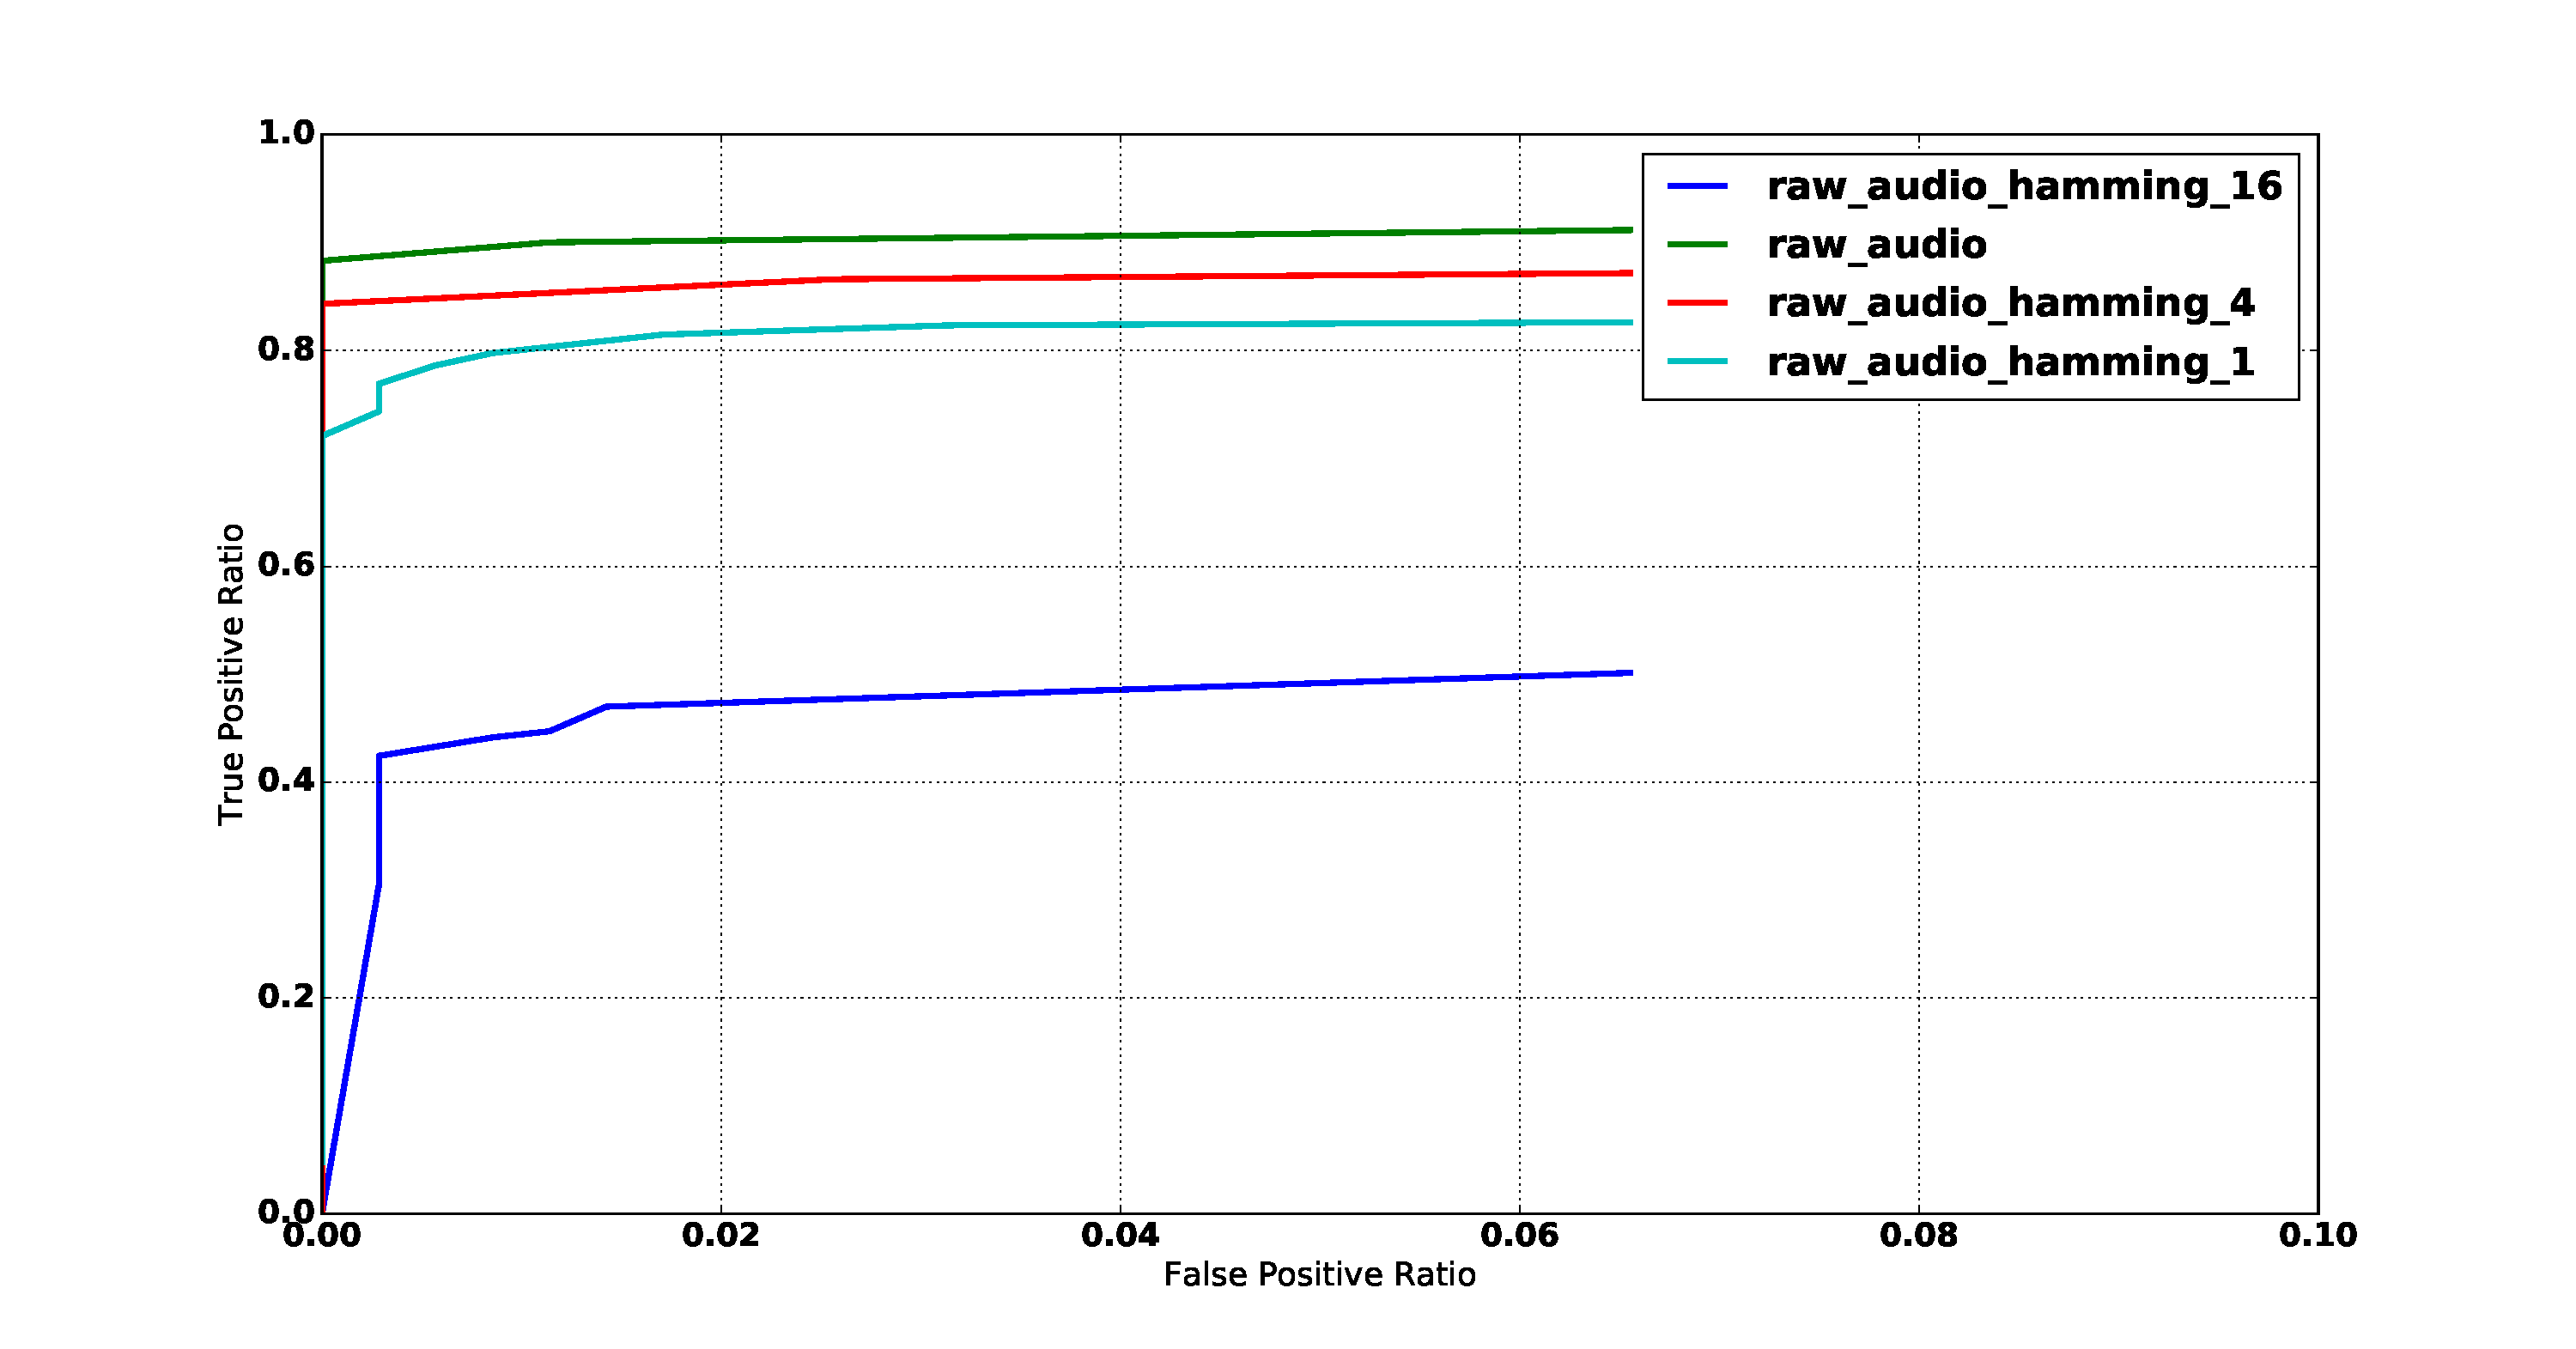
\includegraphics[width=\textwidth]{sound/roc_raw_audio.pdf}
\caption{Receiver Operating Curve (ROC) for Keyphrase Recognition on Raw Audio and Raw Audio obfuscated with Hamming Reduction}
\label{fig:roc_raw_audio}
\end{figure}



\begin{figure}[!th]
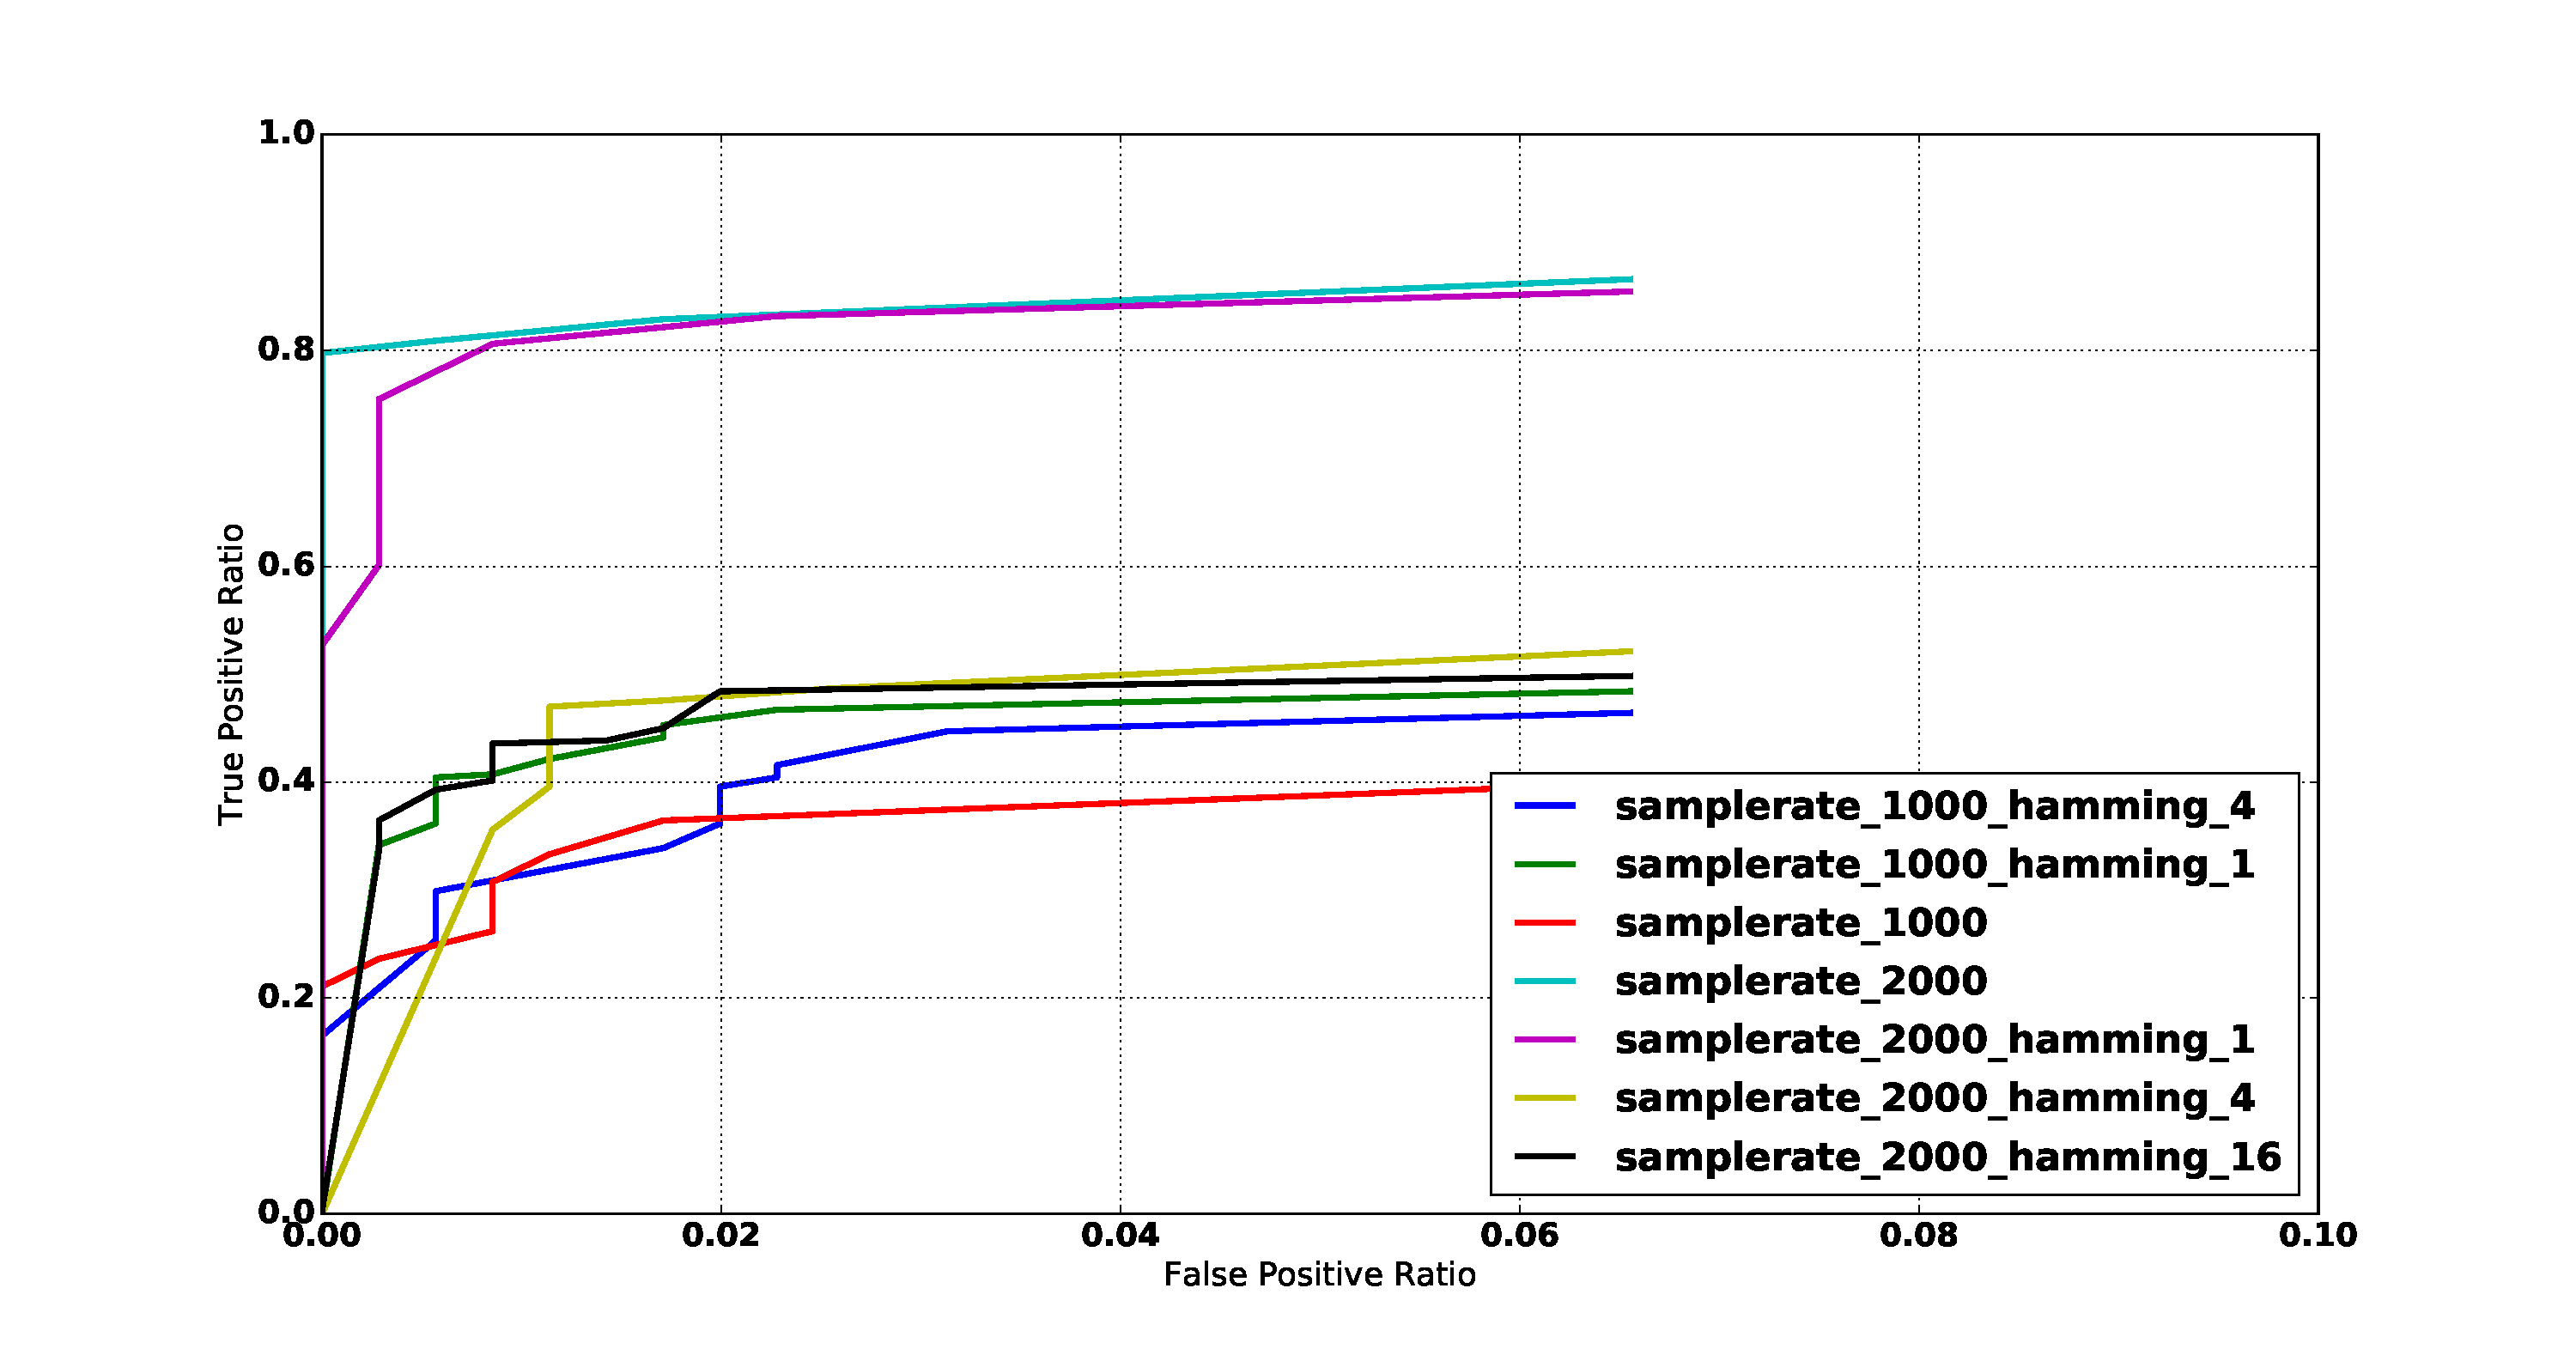
\includegraphics[width=\textwidth]{sound/roc_samplerate.pdf}
\caption{Receiver Operating Curve (ROC) for Keyphrase Recognition on Downsampled Audio and Downsampled Audio obfuscated with Hamming Reduction}
\label{fig:roc_samplerate}
\end{figure}



\begin{figure}[!th]
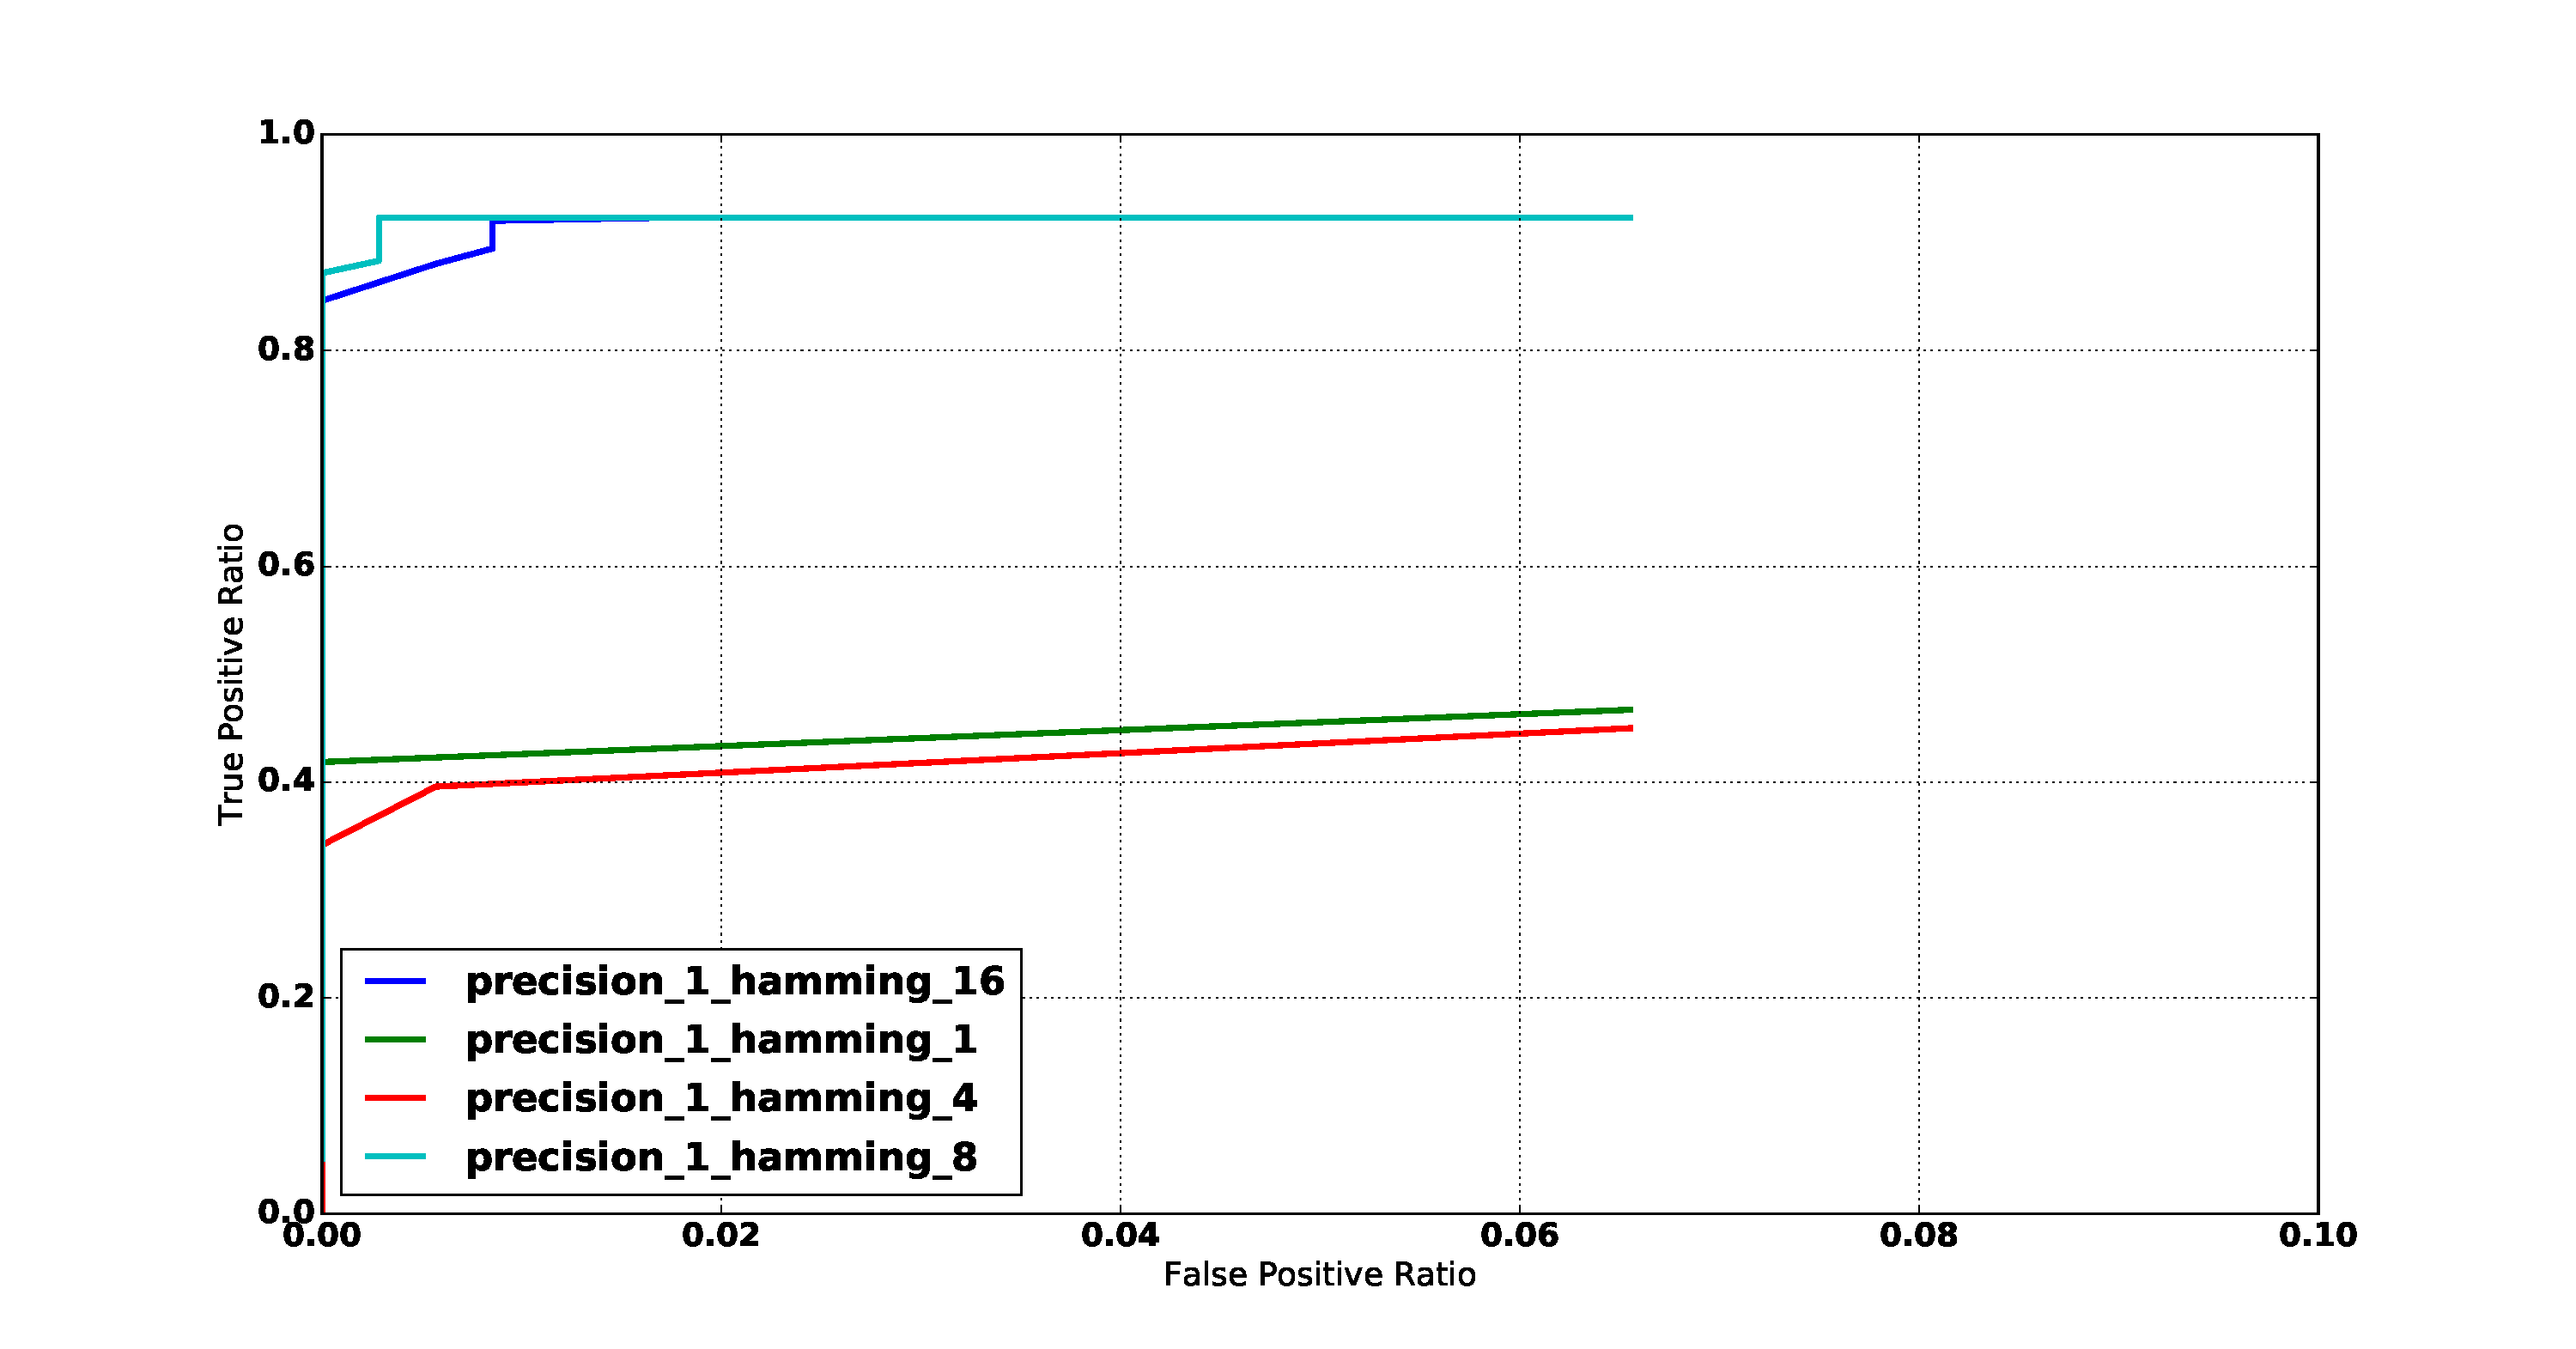
\includegraphics[width=\textwidth]{sound/roc_precision_bits.pdf}
\caption{Receiver Operating Curve (ROC) for Keyphrase Recognition on Low-precision Audio and Low-precision Audio obfuscated with Hamming Reduction}
\label{fig:roc_precision_bits}
\end{figure}




\section{Proposed changes to Mobile Keyphrase Recognition}
\label{sec:proposed_changes_to_mobile}

Using the obfuscated audio technique proposed by the results from the dbHound experimental evaluation, I propose that the Android sensor hub applies the obfuscation to microphone audio and broadcasts it to the applications on the device that wish to provide a voice command interface.
 This model is illustrated in Figure \ref{fig:proposed_voice_command_arch}.
 This way, applications such as browsers wishing to provide simple voice commands (such as "go back", "open new tab" etc.) will not infringe upon the privacy of the user.

\begin{figure}[!t]
\centering
\tikzset{%
    cascaded/.style={%
        general shadow={%
            shadow scale=1,
            shadow xshift=-1ex,
            shadow yshift=1ex,
            draw,
            thick,
            fill=white
        },
        general shadow={%
            shadow scale=1,
            shadow xshift=-.5ex,
            shadow yshift=.5ex,
            draw,
            thick,
            fill=white
        },
        fill=white,
        draw,
        thick,
        minimum width=1.5cm,
        minimum height=2cm
    }
}

\tikzstyle{vecArrowShort}=[thick,
                      shorten >= 5.5pt,
                      postaction={draw,line width=2pt, black, shorten >= 4.5pt}
]
\tikzstyle{vecArrow}=[thick,
                      postaction={draw,line width=2pt, black}
]

\tikzstyle{shortline} = [draw, -latex', fill=black, vecArrowShort]
\tikzstyle{line} = [draw, -latex', fill=black, vecArrow]
\tikzstyle{shortline2} = [draw, dotted, -latex', fill=black, vecArrowShort]
\tikzstyle{line2} = [draw, dotted, -latex', fill=black, vecArrow]

\tikzstyle{input} = [rectangle, draw, fill=green!20, text centered, sharp corners, minimum height=2em, minimum width=15em, align=center]
\tikzstyle{oper} = [rectangle, draw, fill=blue!20, text centered, rounded corners, minimum height=4em, minimum width=10em]
\tikzstyle{output} = [draw, ellipse,fill=red!20, minimum height=2em]

\begin{tikzpicture}[node distance = 2cm, auto]

% nodes
\node [input] (input) { $\text{Microphone}$ };
\node [oper, below of=input] (sensorhub) { $\text{Sensor Hub: Obfuscate Audio}$ };
\node [oper, right of=sensorhub, node distance = 8cm] (dbhound) { $\text{dbHound App}$ };
\node [cascaded, output, below of=sensorhub] (apps) { $\text{Client Applications}$ };

%arrows
\path [line] (input) -- (sensorhub);
\path [line2] (input) -- (dbhound);
\path [shortline] (sensorhub) -- (apps);
\path [shortline2] (dbhound) -- (apps);

\end{tikzpicture}
\caption{Proposed Voice Command Model for Mobile Systems showing dbHound equivalent in parallel}
\label{fig:proposed_voice_command_arch}
\end{figure}



\section{Conclusion}


In this chapter, I present the dbHound system in detail and discuss lightweight obfuscation techniques that can be implemented on mobile devices.
 Based on the experimental data, the most promising obfuscation technique is \texttt{precision\_1\_hamming\_16}.
 In other words, reducing the audio to 1-bit precision and applying the hamming reduce operation over 16 consecutive samples shows the best trade-off between privacy and keyphrase recognition performance.


I envision that such voice-recognition models based on obfuscated audio will provide the solution to maintaining user privacy while improving the accessibility of technology for the physically challenged, as well as providing users with an improved way of interfacing with technology.
